% Remember to save this document with a .Rnw file ending,
% before you use the engine Knitr to compile it.

% ---------------------
% PREAMBLE
% ---------------------
\documentclass{article}\usepackage[]{graphicx}\usepackage[]{color}
%% maxwidth is the original width if it is less than linewidth
%% otherwise use linewidth (to make sure the graphics do not exceed the margin)
\makeatletter
\def\maxwidth{ %
  \ifdim\Gin@nat@width>\linewidth
    \linewidth
  \else
    \Gin@nat@width
  \fi
}
\makeatother

\definecolor{fgcolor}{rgb}{0.345, 0.345, 0.345}
\newcommand{\hlnum}[1]{\textcolor[rgb]{0.686,0.059,0.569}{#1}}%
\newcommand{\hlstr}[1]{\textcolor[rgb]{0.192,0.494,0.8}{#1}}%
\newcommand{\hlcom}[1]{\textcolor[rgb]{0.678,0.584,0.686}{\textit{#1}}}%
\newcommand{\hlopt}[1]{\textcolor[rgb]{0,0,0}{#1}}%
\newcommand{\hlstd}[1]{\textcolor[rgb]{0.345,0.345,0.345}{#1}}%
\newcommand{\hlkwa}[1]{\textcolor[rgb]{0.161,0.373,0.58}{\textbf{#1}}}%
\newcommand{\hlkwb}[1]{\textcolor[rgb]{0.69,0.353,0.396}{#1}}%
\newcommand{\hlkwc}[1]{\textcolor[rgb]{0.333,0.667,0.333}{#1}}%
\newcommand{\hlkwd}[1]{\textcolor[rgb]{0.737,0.353,0.396}{\textbf{#1}}}%

\usepackage{framed}
\makeatletter
\newenvironment{kframe}{%
 \def\at@end@of@kframe{}%
 \ifinner\ifhmode%
  \def\at@end@of@kframe{\end{minipage}}%
  \begin{minipage}{\columnwidth}%
 \fi\fi%
 \def\FrameCommand##1{\hskip\@totalleftmargin \hskip-\fboxsep
 \colorbox{shadecolor}{##1}\hskip-\fboxsep
     % There is no \\@totalrightmargin, so:
     \hskip-\linewidth \hskip-\@totalleftmargin \hskip\columnwidth}%
 \MakeFramed {\advance\hsize-\width
   \@totalleftmargin\z@ \linewidth\hsize
   \@setminipage}}%
 {\par\unskip\endMakeFramed%
 \at@end@of@kframe}
\makeatother

\definecolor{shadecolor}{rgb}{.97, .97, .97}
\definecolor{messagecolor}{rgb}{0, 0, 0}
\definecolor{warningcolor}{rgb}{1, 0, 1}
\definecolor{errorcolor}{rgb}{1, 0, 0}
\newenvironment{knitrout}{}{} % an empty environment to be redefined in TeX

\usepackage{alltt}
\usepackage[sc]{mathpazo}
\usepackage[T1]{fontenc}
%\usepackage[verbose,tmargin=2.5cm,bmargin=2.5cm,lmargin=2.5cm,rmargin=2.5cm]{geometry}
\usepackage[left=25mm,right=35mm,top=25mm,bottom=20mm]{geometry}
%\geometry{verbose,tmargin=2.5cm,bmargin=2.5cm,lmargin=2.5cm,rmargin=2.5cm}
\setcounter{secnumdepth}{2}
\setcounter{tocdepth}{2}
\usepackage{url}
\usepackage[unicode=true,pdfusetitle,
 bookmarks=true,bookmarksnumbered=true,bookmarksopen=true,bookmarksopenlevel=2,
 breaklinks=false,pdfborder={0 0 1},backref=false,colorlinks=true, linkcolor=violet, citecolor=teal]
 {hyperref}
\hypersetup{
 pdfstartview={XYZ null null 1}}
\usepackage{breakurl}

%%%%%% -- PACKAGES WHICH ARE NOT IN THE TEMPLATE -- %%%%%%%%%%%%%%%%
%\usepackage{comment}
\usepackage{fancyvrb}% Verbatim is a more flexible verbatim environment from the package 'fancyvrb'
\fvset{fontsize=\footnotesize, fontfamily=courier} % set font size and family for text in Verbatim environments
\usepackage{natbib}
\usepackage{graphicx}
\usepackage[usenames,dvipsnames,svgnames,table]{xcolor}
\usepackage{framed}
\usepackage{tabulary}
\usepackage{booktabs}
\usepackage{multirow}
\usepackage[format=hang, font=small, labelfont=md]{caption} % package can be used to format captions of all floats in the same way. It overrides any hangcaption/normalcaption commands though.
\usepackage{subcaption}
\graphicspath{ {/Users/Claudius/Documents/PhD/THESIS/kks32/LaTeX/Data_analysis/de-novo-assembly/figures/} }
%% ---- 
\usepackage{float}
\floatstyle{ruled}
\newfloat{command}{htp}{cmd}
%% ----
\usepackage{epigraph} % allows nice quotes with author underneath
\setlength{\epigraphwidth}{.9\textwidth} % set width of quotations to 90% of text width
\renewcommand{\epigraphflush}{center} % centre quotations on the page
\setlength{\epigraphrule}{0pt} % remove the rule under the quote and before the author/source
\renewcommand{\textflush}{flushepinormal} % set to normal justified text
\usepackage{amsmath}
\newcommand{\roger}[1]{ \textcolor[named]{ForestGreen}{#1} }
\usepackage{fancyvrb}

%------ the following package can be used for Word Review function mimicking comments ----------%
\usepackage[textsize=tiny, textwidth=2.5cm, color=Dandelion, colorinlistoftodos]{todonotes} % specify ``disable'' to turn off all notes
\newcommand{\addcit}[1]{\todo[color=yellow!90,nolist]{#1}}
\newcommand{\comment}[1]{\todo[color=green!40,noline,nolist]{#1}}
\newcommand{\longcomment}[1]{\todo[color=green!40,inline,nolist]{#1}}
%\newcommand{\roger}[1]{\todo[color=blue!40]{Roger:\newline{}#1}}
\makeatletter\let\chapter\@undefined\makeatother

%-------------------------------- Glossary ---------------------------------------------
\usepackage{import}

% *** \usepackage[toc,acronym]{glossaries}
% suppress page number list in glossary:
%\usepackage[nonumberlist]{glossaries}

%
% -- put the following code into a .latexmkrc file in the directory from where you run Latexmk --
%
%# add glossary generation to LATEXMK routine
%# ==========================================
%# taken from:
%# http://tex.stackexchange.com/questions/1226/how-to-make-latexmk-use-makeglossaries
%
%add_cus_dep('glo', 'gls', 0, 'run_makeglossaries');
%add_cus_dep('acn', 'acr', 0, 'run_makeglossaries');
%
%sub run_makeglossaries {
%  if ( $silent ) {
%    system "makeglossaries -q $_[0]";
%  }
%  else {
%    system "makeglossaries $_[0]";
%  };
%}
%
%push @generated_exts, 'glo', 'gls', 'glg';
%push @generated_exts, 'acn', 'acr', 'alg';
%$clean_ext .= ' %R.ist %R.xdy';

\makeglossaries

\renewcommand*{\glstextformat}[1]{\textsf{#1}}
%\renewcommand*{\glshyperlink}[1]{\textsf{#1}}

%--------------
% Glossary
%--------------
\newglossaryentry{fragment}{name=fragment, description={not a PCR duplicate. With paired reads from standard RAD (i. e. including random shearing of restriction fragments) typically identified by having different PE read sequences or different insert sizes after read mapping against a reference}}
\newglossaryentry{RAD tag}{name=RAD tag, description={genetic marker from RAD sequencing; the sequence up or downstream of a restriction site}}
\newglossaryentry{barcode}{name=barcode, description={short DNA sequence incorporated into adapter oligonucleotides that becomes part of the sequence read. Barcodes are used in order to be able to pool the DNA of different individuals, populations, treatments, etc. into one library that can be sequenced on one lane of an illumina flow cell}}
\newglossaryentry{index}{name=index, description={similar to barcode and serves the same purpose; generally incorporated into the centre of the adapter so that special sequencing run for the index is required} }
%\newglossaryentry{SbfI}{name=SbfI, description={restriction enzyme with the recognition sequence 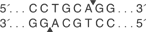
\includegraphics[scale=.5]{Sbf-I-cutsite_1_v1_000015}} }
\newglossaryentry{SbfI}{name=SbfI, description={restriction enzyme with the recognition sequence CCTGCA$\downarrow$GG} }
\newglossaryentry{XhoI}{name=XhoI, description={restriction enzyme with the recognition sequence C$\downarrow$TCGAG} }
\newglossaryentry{heterochromatin}{name=heterochromatin, description={Chromatin that remains in a highly condensed state throughout the cell cycle}}
\newglossaryentry{contig}{name=contig, description={longer consensus sequence derived from assembling smaller overlapping sequence reads}}
\newglossaryentry{linked RAD tag site}{name=linked RAD tag site, description={position in the reference sequence with at least one \gls{concordant} read pair on each side of a putative restriction site and the SE reads overlapping each other as expected from the restriction enzyme}}
\newglossaryentry{proper pair}{name=proper pair, description={read pair from illumina paired-end sequencing that got mapped to a reference in the correct orientation within a maximum expected distance from each other that is determined by the fragment size selection during the sequencing library preparation. Also called a \gls{concordant}ly mapping pair}}
\newglossaryentry{kmer}{name=kmer, description={subsequence with a specified length (k) of a longer sequence}}
\newglossaryentry{e-value}{name=Expect (E) value, description={The Expect value (E) is a parameter that describes the number of hits one can "expect" to see by chance when searching a database of a particular size}}
\newglossaryentry{read}{name=read, description={any sequence that comes out of the sequencer}}
\newglossaryentry{edit distance}{name=edit distance, description={minimum number of operations (one symbol insertion, deletion or substitution) required to change one string of symbols into another. Also known as \emph{Levenshtein distance}}}
\newglossaryentry{Ct}{name={C$_{t}$}, description={PCR cycle when a certain fluorescent threshold is reached}}
\newglossaryentry{mqs}{name={mapping quality score}, description={The mapping quality score \emph{Q} is the Phred transformation of the estimate of the probability \emph{p} that the reported mapping position does not correspond to the read's true point of origin: $Q = -10 \log_{10} p$. The way \emph{p} is estimated is different for each mapping programme, but in any case a mapping quality score \emph{Q} of 3 roughly corresponds to a mis-mapping probability \emph{p} of 0.5, i. e. the read has an estimated 50\% chance to have derived from a location other than the one reported}}
\newglossaryentry{discordant}{name=discordant, description={A read pair is called discordant if it aligns without the expected relative mate orientation (here: forward--reverse or reverse--forward) or outside the expected range of distances between mates. Note that \texttt{bowtie2} only calls discordant read pair mappings if both reads map \emph{uniquely}. Here, I am NOT adopting this requirement}}
\newglossaryentry{concordant}{name=concordant, description={A read pair is called concordant if it aligns with the expected relative mate orientation (here: forward--reverse or reverse--forward) and within the expected range of distances between mates. This is also called a \gls{proper pair}. The complement of \gls{discordant}}}
\newglossaryentry{Levenshtein distance}{name=Levenshtein distance, description={The Levenshtein distance is equal to the minimum number of operations (edits) required to transform one string into another. The allowed operations are single character insertions, deletions and substitutions. This is also known as edit distance.}}
\newglossaryentry{all pairs}{name={all pairs}, description={all the pairs of sequences below a given Levenshtein distance are identified during the graph construction phase}}
\newglossaryentry{transitive clusters}{name=transitive clusters, description={Two read clusters are merged if the distance of any pair of reads between the clusters is below threshold. After merging, the newly created cluster can contain read pairs with distance above the clustering threshold}}
\newglossaryentry{graph}{name=graph, description={A network of connected sequences. Two sequences are directly connected if they match with distance below a threshold. The distance is a measure of the strength of connection, aka "edge weight". Graphs can be stored as a list of pairs of sequences, with an optional edge weight. All graphs here should be "undirected cyclic graphs"}}
\newglossaryentry{Nmer}{name=\emph{N}mer, description={synonymous to kmer, unit, word; a subsequence of size \emph{N} that is overlapping or contiguous with the next subsequence of size \emph{N} and stored in a dictionnary (aka hash) for fast lookup}}
\newglossaryentry{population allele frequency}{name=population allele frequency, description={The population allele frequency is the (unknown) frequency of the allele in the entire population}}
\newglossaryentry{sample allele frequency}{name=sample allele frequency, description={The sample allele frequency is the frequency of the allele among the individuals in a specific sample}}
\newglossaryentry{connected component}{name=connected component, description={All nodes (here sequence reads) after all--pairs search (and before clustering!) that are directly connected by an edge or indirectly connected via several nodes belong to the same connected component} }

%----------------
% Acronyms
%----------------
\newacronym{snp}{SNP}{single nucleotide polymorphism}
\newacronym{rad}{RAD}{Restriction Site associated DNA}
\newacronym{pe}{PE}{paired-end}
\newacronym{se}{SE}{single-end}
\newacronym{bp}{bp}{base pair}
\newacronym{Mbp}{Mbp}{mega base pairs}
\newacronym{Gbp}{Gbp}{giga base pairs}
\newacronym{indel}{indel}{small sequence insertion or deletion polymorphism}
\newacronym{SAM}{SAM}{Sequence Alignment/Map format}
\newacronym{EST}{EST}{expressed sequence tag}
\newacronym{ddRAD}{ddRAD}{double digest RAD}
\newacronym{ML}{ML}{maximum likelihood}
\newacronym{SFS}{SFS}{site frequency spectrum}
\newacronym{HWE}{HWE}{Hardy Weinberg equilibrium}
\newacronym{CI}{CI}{confidence interval}
\newacronym{EM}{EM}{Expectation Maximisation}
\newacronym{DEM}{DEM}{digital elevation model}
%-------------------------------- Glossary ---------------------------------------------


% -----------------------------------------------------------------------------------

% -----------------------
% DOCUMENT
% ------------------------
\IfFileExists{upquote.sty}{\usepackage{upquote}}{}
\begin{document}

% ----------- -- KNITR SETUP -- -------------------------

% ----------------------------------------------------------------



\title{De novo assembly of RADseq data}


\author{Claudius Kerth}

\maketitle

\abstract{Here I document different approaches to the de novo assembly of RADseq data.}

%\listoftodos

\section{Introduction}

\cite{Ilut2014} describe an empirical method to determine the \textbf{optimal within cluster distance} for RAD tag de novo assembly. Using digital digests of several genome sequences with one restriction enzyme (but without random shearing, i. e. equivalent to double--digest), they create a clustering threshold series with 1--haplotype, 2--haplotype and $\ge$3--haplotype cluster number curves. They create a \gls{graph} with \href{http://cbrc3.cbrc.jp/~shimizu/slidesort/index.php?SlideSort}{\texttt{SlideSort}} from all distinct input sequences and then create \gls{transitive clusters} with different distant thresholds.

\cite{Shimizu2011} have developed \href{http://cbrc3.cbrc.jp/~shimizu/slidesort/index.php?SlideSort}{SlideSort} for clustering reads of almost identical length. It is very time and memory efficient and due to alignment by dynamic programming of candidate pairs \textbf{it allows for indels as well}. \texttt{SlideSort} is based on a pattern growth algorithm that can effectively narrow down the search by finding chains of common k--mers. This algorithm seems to be much more efficient than single-seed/k-mer based algorithms as employed in stacks. \texttt{SlideSort} also provides an undirected graph $G$, where vertices/nodes represent reads and weighted edges represent edit distances of neighbour pairs. This graph can be fed into a separate clustering programme. \texttt{SlideSort} can also make use of multiple cores.

\cite{Ilut2014} propose that the optimal cluster distance threshold is where the 1--haplotype and 2--haplotype clusters start to plateau and the $\ge$3--haplotype clusters are still low in proportion. Higher thresholds would not increase the detection of heterozygous loci much while increasing the proportion of paralogous sequences within the 2--haplotype cluster category. Since finding distant sequence matches is computationally demanding\todo[nolist]{Running slidesort for 134,492 distinct sequences from ery\_30-10 took 2h19min on a single core. But \texttt{SlideSort} is parallelised.}, they show that subsets of the data (30\% or more) already produces the same curves as the whole data set. They also recorded the pairwise distance between all reads\footnote{this can be a very large matrix} for the clustering with the highest threshold to be tested and limited the transitive re-clustering for lower thresholds to those read pairs that have a recorded distance $\le$ to the highest threshold in the test series\todo[nolist]{They read the edges weights from \texttt{slidesort} into a hash (see \texttt{slidesort\_cluster.pl}). So only looking up sequences within a specified max distance is trivial.}. 

They also show that RAD data from a highly polymorphic gene pool is expected to contain a large proportion of loci affected by \textbf{null alleles} due to polymorphisms in the restriction site(s), a possible issue which affects RAD protocols without random shearing much more (i. e. two complete restriction sites necessary to sample an allele) than with random shearing. \cite{Ilut2014} also derive the number of reads required per locus and individual in order to reduce the probability of sampling only one allele from a heterozygous locus (see their supp. mat.). For instance, using their formula (iii) and setting the minimum allele coverage to 2\footnote{which is the absolute minimum to prevent sequencing errors from being called alleles}, the required per individual and locus minimum coverage in order to reduce the proportion of false homozygous calls due to binomial sampling of alleles to 5\% is 9x! If we are, however, only randomly choosing one allele per RAD tag genotype call, then we can include loci where individuals have a coverage below this minimum threshold. We should even derive a genotype probability distribution even when there is \emph{no} read from an individual at a given locus (i. e. using only information from other individuals from the same population in a hierarchical Bayesian model)! 

%\textit{Another question is the relevance of having to determine the optimum within locus distance threshold for clustering given the performance of naive clustering programmes like \href{www.micans.org/mcl/}{\texttt{MCL}} that find "intrinsic" clusters in the read data as used in the Peterson pipeline (see below and \citealt{Peterson2012})\todo[nolist]{\texttt{MCL} requires optimisation of the inflation parameter in order to find clusters at the right hierarchical level!}.} Adjustment of the inflation parameter to \texttt{MCL} will be necessary in order to obtain mainly the clusters at the right level (i. e. alleles instead of paralogs). 


% --------------------------------------------------
\subsection{Testing the Ilut pipeline}
% --------------------------------------------------
I got the Ilut pipeline scripts (in Perl) from Dan Ilut and ran it on the standard RAD SE reads (\texttt{stacks} quality cleaned) of one individual: ery\_30-10. The reads are 46 bp long, but the first 6 bp are the remainder of the SbfI site. I let the pipeline collapse all reads into distinct sequences and keep only those with a read count of at least 2. I specified a maximum edit distance for \texttt{SlideSort} of 8, which corresponds to a 20\% divergence, and disabled \emph{gap-postprocessing}\todo{this is an interesting feature, but it is much more compute intensive}~by the Ilut pipeline. The implied scoring scheme is therefore -1 for every mismatch and -2 for every base pair of indel (global alignment). See the file \texttt{template-parameters\_for\_run} that contains an explanation for each pipeline parameter. The log file in the output directory documents very well what the pipeline has done, including the command lines it executed. \texttt{Slidesort} clustering of 134,492 distinct sequences with a maximum edit distance of 8 took 2h 20min. \texttt{Slidesort} outputs a graph specifying each edge in the standard \texttt{seqID,seqID,edit distance} format. \texttt{Slidesort} is only run once for the maximum edit distance. Clusters for all edit distances up to this maximum can then be inferred from the \texttt{Slidesort} graph output. This is done by the pipeline script \texttt{slidesort\_cluster.pl}, which transitively (i. e. recursively) clusters reads. I did not apply an extra filtering of clusters for minimum coverage, that is 2 reads for a singleton cluster (putative homozygous locus) was enough to retain the cluster.%\todo{I think for the de novo assembly with reads of one individual, I should require 2 reads per allele, i. e. 4 reads per locus.}
~The Ilut pipeline also contains a cluster filtering script (\texttt{sort\_depth\_cols.pl}), which requires a specific distinct sequence in a cluster to contribute a minimum proportion towards the total read count of the cluster. I set this to 0.05. I documented the analysis of the output of the Ilut pipeline on huluvu in \\ \texttt{/data3/claudius/Ilut\_pipeline/Ilut\_output/ery\_30-10\_1459448900/Optimal\_Dist\_Threshold.Rmd}.

\begin{figure}
\centering
\includegraphics[width=\textwidth]{distance-threshold-1}
\caption{Distance threshold series from the Ilut pipeline. The number of distinct sequences in clusters of size 1, 2 and $\ge$3 are plotted for each maximum edit distance threshold for transitive clustering.}
\label{Fig:Ilut-Distance-threshold-series}
\end{figure}

\comment{
Further things to look at are:
\begin{itemize}
\item improvement of gap scoring 
\item low complexity filtering of input sequences to the clustering software
\item minimum coverage filtering
\item high coverage filtering
\end{itemize}
}

Figure \ref{Fig:Ilut-Distance-threshold-series} shows the outcome of transitive clustering with different maximum edit distances by the Ilut pipeline. Note that I am plotting the number of distinct sequences in each cluster size category instead of simply the number of clusters in each size category as in \cite{Ilut2014}. The first striking outcome is the invariance of the number of 2--haplotype clusters with respect to the maximum distance threshold for clustering: a maximum edit distance of just 1 collapses already as many sequences into 2--haplotype clusters as a maximum edit distance of 8. The second striking outcome is the invariance of the number of clusters with 3 or more sequences with respect to the cluster distance threshold. This invariance is due to the cluster filtering script \texttt{sort\_depth\_cols.pl}, which processes the raw clusters and removes all \emph{sequences} from clusters which contribute less than 5\% to the total read count of the cluster. Remarkably, this simple filtering criterion removes all \emph{clusters} with more than 12 sequences (fig. \ref{Fig:raw-cluster-size-distribution-maxD8-1}).

\begin{figure}
\centering
\includegraphics[width=\textwidth]{raw-cluster-size-distribution-maxD8-1}
\caption{Cluster size distributions before (top) and after (bottom) filtering with \texttt{sort\_depth\_cols.pl} and a minimum read proportion of 5\% for every sequence in a cluster.}
\label{Fig:raw-cluster-size-distribution-maxD8-1}
\end{figure}

The third (less striking) outcome is that with a bigger cluster distance threshold the number of 1--haplotype clusters decreases. One would  expect that 1--haplotype clusters get merged into 2--haplotype clusters and that this would increase the number of 2--haplotype clusters. Clearly, that is not the case. Is the rate of 2--haplotype cluster formation with increasing cluster distance threshold the same as the rate of merging 2--haplotype clusters into or with paralog clusters? Yes! As can be seen in figure \ref{Fig:movement-between-cluster-sizes-1}, the largest movement of sequences between cluster sizes when increasing the cluster distance threshold is by sequences in 1-haplotype clusters to paralog clusters. The population of 2-haplotype clusters is by no means stable. The \emph{number} of 2-haplotype clusters is so stable because the rate of creation of 2-haplotype clusters from two 1-haplotype clusters is very similar to the rate of creation of paralog clusters ("3+") from 2-haplotype clusters. So this cluster size category happens to gain about as many sequences as it looses for each increase in cluster distance threshold.

\begin{figure}
\centering
\includegraphics[width=.8\textwidth]{movement-between-cluster-sizes-1}
\caption{Movement of sequences between cluster size categories as the cluster distance threshold is varied for transitive clustering. For instance, the uppermost and leftmost point indicates that there are 13,000 sequences that are in 1--haplotype clusters at distance threshold 1 and then "move" to 3+--haplotype clusters at distance threshold 2.}
\label{Fig:movement-between-cluster-sizes-1}
\end{figure}

% ------------------------------------------------------------------------------------------------
\subsection{Which cluster distance threshold is optimal then?}
% ------------------------------------------------------------------------------------------------
So, neither the 1--haplotype nor the 2--haplotype cluster size categories seem to converge towards an asymptote within the maximum cluster distance threshold of 8 (fig. \ref{Fig:Ilut-Distance-threshold-series}). Additionally, there seems to be a continuous movement of sequences between cluster size categories when increasing the cluster distance threshold from 1 to 8 (fig. \ref{Fig:movement-between-cluster-sizes-1}). The edit distance of 8 that I specified for this pipeline corresponds to 20\% divergence for the variable sequence length of these reads: 40 base pairs. Probably one of the largest \emph{average} allelic pairwise divergence estimates was found in the sea squirt \textit{Ciona savignyi}: 5\% \citep{Small2007}. The nucleotide diversity in 4-fold degenerate sites is even 8\% in this species. According to this, if I would take the edit distance of 8 as cluster distance threshold, I should to a large extent already cluster paralogous sequences. 5\% divergence would correspond to an edit distance of 2 with these reads. So, if I was to allow up to 4 edits between alleles (i. e. 10\% divergence) I should be able to cluster more than 99\% of alleles (see text for fig. 2 in \citealt{Small2007}). 

Figure \ref{Fig:dist-between-alleles}a shows the distribution of divergence between alleles (haplotypes) in putative loci reconstructed with maximum cluster distance of 8. 
Under mostly neutral evolution and assuming that the infinite-sites model of mutation without recombination holds for these sequences, this distribution of edit distances (or \emph{number of segregating sites $S$}) between alleles should roughly follow a geometric distribution with parameter $p$ equal to $\frac{1}{\theta +1}$ ($\theta$ being the per locus mutation parameter $2N_{e}\mu$) and multiplied by the total number of loci \citep[sec. 4.1.1 ]{Wakeley2009}.

\begin{align}
P\{S=k\} \times \text{n\_loci} &= \left( \frac{1}{\theta+1} \right) \left( \frac{\theta}{\theta+1} \right)^{k} \times \text{n\_loci}
\end{align}


This prediction is based on the assumptions that:
\begin{enumerate}
\item I have taken an identical sample size from each locus (2), 
\item that I have sampled many independent loci 
\item and that all loci have the same underlying value of $\theta$.
\end{enumerate}

It is unlikely that any of these assumptions is fully met. Allele dropout due to binomial sampling of alleles during library preparation and sequencing as well as polymorphisms in the restriction site will lead to a violation of the first assumption. Any linkage disequilibrium between RAD tag loci will reduce the effective number of loci sampled and linkage with  loci under varying degrees of selection will violate the third assumption. However, I think the effect of allele dropout on the distribution will be somewhat counteracted by the clustering of paralogous sequences and I am assuming that their divergence can also be modelled by the geometric distribution (duplication being equivalent to coalescence\todo[nolist]{But duplications are much rarer than coalescences. So if the divergence of paralogs can also be modelled by a geometric distribution, then their parameter $p$ should be much smaller.}). I think the violations of assumption 2 and 3 will be noticeable but less severe.

\begin{figure}
\large
\centering
\hspace{-400pt}a)\\
\includegraphics[width=.9\textwidth]{dist-between-alleles-1-1}
\vspace{20pt}\\
\hspace{-400pt}b)\\
\includegraphics[width=.9\textwidth]{dist-between-alleles-2-1}
\caption{Distribution of divergence between haplotypes in putative homozygous and heterozygous clusters with a maximum cluster distance of 8. Expected distributions are plotted for comparison. Subfigure b) zooms in on the counts in the higher edit distance categories. In this geometric regression, I have assumed that all loci have haplotypes with edit distance between 0 and 8. The very few loci with more distant haplotypes will be counted in the 0-edit distance category.}
\label{Fig:dist-between-alleles}
\end{figure}

The observed distribution of edit distances between putative alleles would fit best to a $2N_{e}\mu_{locus}$ value of 0.102\todo{It would be good to get a posterior distribution of $\theta$ instead of just a ML estimate.}~(per locus) or 0.00256 per nucleotide site. So as expected much lower than the value estimated for \textit{Ciona savignyi} (fig. \ref{Fig:dist-between-alleles}a). It seems likely that the 0-edit-distance category (i. e. putative homozygous loci) is inflated due to allele dropout because of polymorphisms in the restriction site and low coverage that makes heterozygous loci appear homozygous.. However, a lower number of homozygous loci would imply a higher $\theta$ and this would imply a much higher count of heterozygous loci with 1-edit distance (see red curve in fig. \ref{Fig:dist-between-alleles}a). The edit distance categories from 4\ldots8 are all much higher than expected by any reasonable $\theta$ (see fig. \ref{Fig:dist-between-alleles}b). This could be due to clustering of paralogs. However, since I am looking at 1-- and 2--haplotype clusters here, this clustering of paralogs would also tend to reduce the 0--edit--distance (i. e. 1--haplotype) category. All reads for the clustering had a minimum read count of 2, so sequencing error should not significantly inflate the higher edit distance categories. It must be noted that these are still raw clusters, i. e. they have not undergone any filtering yet\todo{I should therefore redo this analysis after filtering. The goal should be to improve the fit to a geometric distribution. I should also filter the input reads for low complexity sequences. This might additionally improve the results.}.~

If the observed distribution of pairwise differences between alleles would follow a geometric distribution, then the average number of pairwise differences $\pi$ would be equal to $\theta$. The average number of pairwise differences is 0.345, so about 3 times higher than the geometric regression estimate. This estimate is likely an overestimate, since it results from the heavy tail of the observed distribution which is likely to contain clusters of paralogous sequences.

For details of this analysis, see \texttt{Optimal\_Dist\_Threshold.Rmd} in \\ \texttt{/data3/claudius/Ilut\_pipeline/Ilut\_output/ery\_30-10\_1459448900} on huluvu.


%----------------------------------------------------
\subsection{Clustering of all--pairs graphs with dedicated clustering programmes}
%----------------------------------------------------

The transitive clustering of the Ilut pipeline (by \texttt{slidesort\_cluster.pl}) returns all connected networks of sequences from a graph. It thereby returns the largest possible clusters where each edge within a cluster has a weight less than or equal to a specific maximum distance threshold and it ignores any structure within these clusters. For instance, when clustering a graph with maximum edge distance of 8, there could be a network of three sequences A, B and C. A and B could be 1 mutation apart and C 8 mutations apart from B.\todo{insert a simple sketch here with TikZ}~There is therefore clearly substructure in this network. There are a range of clustering programmes (mainly aimed at clustering protein sequences from different species) that can recognise this substructure (i. e. remove the edge from B to C) when given a suitable density parameter (aka as \emph{inflation} parameter in \texttt{MCL}). I tried out the clustering programme \href{http://micans.org/mcl/}{\texttt{MCL}} with graphs from \texttt{starcode} and \texttt{blastn}. I varied the inflation parameter and analysed the resulting clusterings. A detailed documentation is in two Rmarkdown files on huluvu\todo{create a graph from the per individual uniqued sequences of all individuals of one population and analyse cluster size distributions for different similarity thresholds}: 
\begin{itemize}
\item[\emph{starcode}] \texttt{/data3/claudius/graph\_construction/MCL\_clustering/MCL\_inflation\_variation.Rmd}
\item[\emph{blast}] \texttt{/data3/claudius/MCL/clustering/ery\_30-10/MCL\_inflation\_variation\_blast.Rmd}
\end{itemize}

\cite{Zorita2015} describe a new \gls{all pairs} graph construction algorithm. Their programme \href{https://github.com/gui11aume/starcode}{\texttt{starcode}} finds all pairs of sequences within a specified \gls{Levenshtein distance}. It uses a modified \href{https://en.wikipedia.org/wiki/Needleman\%E2\%80\%93Wunsch_algorithm}{Needleman--Wunsch algorithm} (global alignment) during a depth--first search on a prefix tree after seed filtering. Because edit distance is determined from a global alignment, \texttt{starcode} should be provided with sequences of equal length, otherwise length differences will be counted as gaps and thereby increase edit distance. Their scoring scheme is 0 for a match and 1 for a mismatch, insertion or deletion. Note, that when read length has a strict limit, an insertion within the read will cause \emph{two} gaps of equal lengths when matched against a sequence without that insertion: one within the read and one at the end (due to the limit in read length). Practically that means that indels get twice the penalty as substitutions with the NW algorithm. \texttt{starcode} is parallelised. 

\texttt{starcode} can be set to find pairs of sequences within a maximum number of mismatches of 1$\dots$8. That could be limiting for 200 bp long reads but might be due to the exponential increase in running time with increase in allowed mismatch. Although they don't show it, but I suspect that the bigger problem might be the memory footprint with higher allowed distance threshold (see their table 5 showing maximum memory usage on real datasets and a distance threshold of only 3). \texttt{starcode} does not only produce a graph, it also implements two different clustering algorithms, which determine canonical sequences (aka centroids) from the reads with the highest read count. \texttt{starcode} returns the canonical sequence for each cluster, the cluster size\footnote{it seems that the cluster size is not correctly reported, see my issue on github} and a list of the (unique) sequences that form the cluster. This is a very useful output that I can easily use for filtering. The \texttt{starcode} authors also show that \texttt{SlideSort} is not an all--pairs search algorithm as it does not find all sequence pairs up to a given threshold (see \href{https://github.com/gui11aume/starcode/tree/master/misc}{here} for a proof). {\bfseries So, \texttt{SlideSort} seems to be buggy!} On a putative RNA--seq dataset, \texttt{starcode} seems to be orders of magnitudes faster than SEED and CD--HIT--est on the task of clustering with a threshold of 3. \texttt{SlideSort} fails completely! 

\texttt{starcode} has a git branch called \texttt{allpairs} whose version of starcode prints out edges without clustering, i. e. "seq1 seq2 distance" for all pairs of input sequences that are within the specified edit distance. This format can be used by clustering programmes like \texttt{MCL} .

Like for the Ilut pipeline, I have run \texttt{starcode} on SE reads of one individual from the Big Data set. I have first collapsed these reads into unique sequences and only retained sequences with read count $\ge$2. Only about 2\% of input reads (already \texttt{stacks} quality filtered) were singletons. The reads are 46 bp long including the 6 bp long remainder of the SbfI restriction site at the beginning of each read. Therefore, an edit distance of 8 corresponds to a divergence of 20\%! I have then fed these 134,492 distinct sequences into \texttt{starcode} specifying a distance of 8, \emph{all pairs} mode\footnote{programme version from its \emph{allpairs} git branch} and parallelisation with 12 threads. \texttt{starcode} was finished after just 3 minutes with negligable memory usage. 

The "abc" format from \texttt{starcode} was then read into \texttt{MCL} to create a matrix. Since \texttt{MCL} takes similarities as edge weights and \texttt{starcode} outputs distances between read pairs, I linearly transformed the distances simply with "similarity = 9 - distance". Therefore, a distance of 8 would become a similarity of 1 and a distance of 1 would become a similarity of 8. I then created a similarity threshold series on the \emph{un}clustered \texttt{starcode} graph using a utility programme that comes with \texttt{MCL}: \texttt{mcx query}. This command allows the application of different levels of similarity thresholds on a graph and it provides information about the resulting graph. Increasing the similarity threshold obviously leads to the removal of edges and therefore the split up of clusters. This is exactly what the script \texttt{slidesort\_cluster.pl} in the Ilut pipeline does. I have applied a similarity threshold series from 1 till 8. Figure \ref{Fig:similarity-threshold-series-starcode-1} shows the similarity threshold series for the \texttt{starcode} graph. 
\begin{figure}[!htb]
\centering
\includegraphics[width=.9\textwidth]{similarity-threshold-series-starcode-1}
\caption{Distribution of the number of sequences (here called \emph{nodes}) in clusters of size 1, 2 and $\ge$3 over the range of similarity thresholds (here called \emph{edge weight cutoff}) applied to edges in the \texttt{starcode} graph. There were 38,421 sequences that had no match within edit distance of 8 and therefore did not appear in the \texttt{starcode} graph. I have added their number to the cluster size category 1.}
\label{Fig:similarity-threshold-series-starcode-1}
\end{figure}
Note that this figure shows the same as figure \ref{Fig:Ilut-Distance-threshold-series} for the \texttt{Slidesort} graph. Only the x--axis needs to be inverted to make them the same. Nodes are the same as distinct sequences. After inversion of the x--axis, the curves for cluster size 1 and 2 are practically identical for the two figures! The number of sequences in paralogous clusters is much higher in figure \ref{Fig:similarity-threshold-series-starcode-1} than figure \ref{Fig:Ilut-Distance-threshold-series}, since the Ilut pipeline also applies a filter on clusters (by its script \texttt{sort\_depth\_cols.pl}) that removes sequences from clusters that contribute less than 5\% of coverage to the total coverage of the cluster, which as figure \ref{Fig:raw-cluster-size-distribution-maxD8-1} shows removed all clusters of size greater 9. The symmetry of the 1--allele and $\ge$3 curves in figure \ref{Fig:similarity-threshold-series-starcode-1} suggest that new 1--allele clusters split off paralog clusters when increasing the similarity threshold. Figure \ref{Fig:movement-between-cluster-sizes-1} confirms this.

As stated above, similarity or distance thresholds are a rather crude way to manipulate the granularity of a graph. Clustering algorithms can find intrinsic structure in graphs without applying a one--for--all threshold for edge weights. All clustering programmes, however, require  at least one parameter that specifies the degree of granularity. In \texttt{MCL} this parameter is called \emph{inflation} parameter, in \texttt{TransClust} \emph{density} parameter. A low inflation parameter leads to coarse clustering, a high inflation parameter leads to smaller clusters. I therefore clustered the \texttt{starcode} graph with \texttt{MCL} and a series of different inflation parameters.  
\begin{figure}
\centering
\includegraphics[width=.9\textwidth]{inflation-variation-1}
\caption{Distribution of cluster counts (not sequence counts as in previous plots!) in different size categories over different inflation parameters for \texttt{MCL}. The lowest possible inflation parameter for \texttt{MCL} is 1. The points at inflation 0 represent the cluster sizes in the unclustered \texttt{starcode} graph.}
\label{Fig:inflation-variation-1}
\end{figure}
Figure \ref{Fig:inflation-variation-1} shows the outcome of MCL clustering with different inflation parameters. The greatest change in the number of clusters of size 2 occurs for inflation parameters between 1 and 2. Almost 1,000 new 2--allele clusters are created by \texttt{MCL} with an inflation parameter of 2 compared to the baseline (no clustering). At the same time, only very few 1--allele clusters are created. This is a great behaviour, since I want to split 2--allele clusters off paralog clusters without splitting 2--allele clusters apart.
The ratio between 2--allele and 1--allele clusters could therefore be used as an optimality criterion. 
\begin{figure}
\centering
\includegraphics[width=.9\textwidth]{clustering-score-1}
\caption{Distribution of clustering score over the different inflation parameters. The score is simply the number of clusters in size category 2 (putative heterozygous loci) divided by the number of newly created clusters in size category 1 (putative homozygous loci or alleles).}
\label{Fig:clustering-score-1}
\end{figure}
Figure \ref{Fig:clustering-score-1} shows this score for the different clusterings. Since the number of \emph{class 1} clusters is still very low, an inflation parameter of about 2.0 could be optimal.

As with the \texttt{Slidesort} graph, I can extract the distances between putative alleles from the unclustered \texttt{starcode} graph and the \texttt{MCL} clusterings with different inflation parameter. 
\begin{figure}
\centering
\includegraphics[width=.9\textwidth]{allele-distance_dist-starcode-unclustered-1}
\caption{Distribution of edit distances between putative alleles from the unclustered \texttt{starcode} graph. The expectations of counts from the geometric regression are plotted on top.}
\label{Fig:allele-distance_dist-starcode-unclustered}
\end{figure}
Figure \ref{Fig:allele-distance_dist-starcode-unclustered} shows the distribution of pairwise differences between sequences in 1-- and 2--haplotype clusters of the unclustered \texttt{starcode} graph. Since \texttt{starcode} and \texttt{Slidesort} have produced a practically identical graph from the same set of sequences, the ML estimate of $\theta$ is also practically the same. So far, so unsurprising. But how does \texttt{MCL} clustering affect the distribution of pairwise differences in 1-- and 2--haplotype clusters?
\begin{figure}
\centering
\includegraphics[width=.9\textwidth]{allele-distance_dist-starcode-clustered-1}
\caption{Distribution of edit distances between putative alleles from the cluster output of \texttt{MCL} run with different inflation parameters. The plot zooms in on the counts for edit distances greater 0.}
\label{Fig:allele-distance_dist-starcode-clustered}
\end{figure}
Figure \ref{Fig:allele-distance_dist-starcode-clustered} shows the distribution of pairwise divergence between sequences of 1-- and 2--haplotype clusters from \texttt{MCL} clusterings with different inflation parameters. A finer clustering with higher inflation parameter leads to a conspicuous increase in the counts for the largest two edit distances. This speaks against fine clustering. It seems to split off pairs of highly divergent sequences from paralog clusters.\todo{The ratio of increase (compared to the baseline) in the 1--edit--distance class to the increase in the 8--edit--distance class could be an optimality criterion.} ~
\begin{table}[htdp]
\centering
\caption{ML $\theta$ estimates from geometric regressions to pairwise allele distance distributions from different \texttt{MCL} clustering with different inflation parameters.}
\begin{tabular}{ccc}
inflation parameter & ML $\theta$ & $R^{2}$ \\
\toprule
1.0 & 0.102 & 0.9966 \\
1.6 & 0.114 & 0.9959 \\
5.0 & 0.131 & 0.9942 \\
15.0 & 0.138 & 0.9930 \\
\bottomrule
\end{tabular}
\label{Tab:inflation-theta}
\end{table}%
The $\theta$ estimates are surprisingly different given the similarity of the distributions of edit distances from different clusterings (tab. \ref{Tab:inflation-theta}). If I were to choose the inflation parameter that produces the best fit to a geometric distribution with the ML estimate of $\theta$, I would have to choose 1.0, which is equivalent to no clustering at all (see $R^{2}$ in tab. \ref{Tab:inflation-theta}). Any clustering reduces the fit to a corresponding geometric regression.

For the details of this analysis see: \\
\texttt{/data3/claudius/graph\_construction/MCL\_clustering/MCL\_inflation\_variation.Rmd} on huluvu.


\comment{Could \emph{low complexity} filtering, for instance during blast database construction, improve clustering results?}
\comment{I should do a separate assembly for each subspecies, to make it easier for \texttt{MCL} to distinguish orthologs from paralogs.}

%----------------------------------------------------------------------------------------------------------------------------------
\subsection{Analysis of all--pairs graphs created with sequences from a whole population}
%----------------------------------------------------------------------------------------------------------------------------------

%----------------------------------------------------------------------------------------------------------------------------------
\subsubsection{When I create clusters with any programme, should I expect a large fraction of loci sampled from one population to be monomorphic?} 
%----------------------------------------------------------------------------------------------------------------------------------
Roughly how big should that fraction be given a certain nucleotide diversity ($\theta$), sample size (binomial), read length (40) and rate of allele dropout (unknown)? 

Equation 4.3 in \citep[p. 43]{Wakeley2009} gives the generalisation of the $P\{S=k\}$ for a sample of $n$ alleles:
\begin{align}
P\{S=k\} &= \sum_{i=2}^{n} (-1)^{i}\binom{n-1}{i-1}\left(\frac{i-1}{\theta+i-1}\right)\left(\frac{\theta}{\theta+i-1}\right)^{k}
\end{align}

I want to solve this equation for $k=0$ and using the ML estimate for $\theta$ from above, but now with a higher number of $n$ than 2. I do not expect that I will get a minimum of 2 reads (minimum coverage for detection) from every allele at every locus from each individual. I therefore tried to model the number of sampled alleles at a locus with $n\sim binom(36, 0.5)$. 36 is the number of alleles in a sample of 18 diploid individuals and 0.5 is the probability of getting 2 reads from an allele at a locus from an individual. So I am expecting to sample on average only half the gene copies at a locus in the sample of 18 individuals. This could even be an optimistic expectation. I thus simulated the sampling of 10,000 loci and calculated for each the probability of zero observed segregating sites among the sampled alleles. Figure \ref{Fig:prop-monom-clust-1} shows the probability density distribution of the proportion of monomorphic loci (clusters) that resulted from this simulation.
\begin{figure}
\centering
\includegraphics[width=.9\textwidth]{prop-monom-clust-1}
\caption{The probability density that there are no segregating sites among a sample of $n$ alleles given $\theta$. The number of sampled alleles is assumed to be binomially distributed with a total of 36 alleles from which $n$ alleles are chosen, each with a probability of 0.5. The 90\% equal tail interval is shown in blue.}
\label{Fig:prop-monom-clust-1}
\end{figure}
So, I should be expecting a little bit less than 70\% of loci to be monomorphic. Note, that this estimate does not incorporate my statistical uncertainty about $\theta$. For those monomorphic samples of gene copies, each individual for which at least one allele was sampled will contribute 1 to the cluster size count.


\cite{Roettger2013} describe an interesting approach to optimising the density parameter for their clustering programme \texttt{TransClust}. They use whole genome protein sequences from 89 bacterial species and cluster them with a range of density parameters. They then choose the density parameter that:
\begin{enumerate}
\item achieves the highest number of clusters with size 89 and 
\item the lowest number of clusters containing more than 89 sequences
\end{enumerate}
This approach could be useful for clustering sequences from all 18 individuals of one population if I can expect a distinct peak of a certain cluster size at or around the true cluster size. In contrast to \citealt{Roettger2013}, I have a varying sample size for each locus due to insufficient coverage. This also means that, unless I sample two different alleles, I cannot know whether an individual is really homozygous or whether it is heterozygous and I only sampled one of the two alleles. I collapse identical reads into one unique sequence per individual before clustering. So each distinct allele adds 1 towards the cluster size. If I sample two different alleles in an individual, they would obviously add 2 toward the cluster size. 

It would be good to get an estimate of the expected distribution of cluster sizes. This distribution will depend on the number of alleles sampled from each individual (0, 1 or 2) and if 2 alleles were sampled, whether these alleles are different. The probability that two alleles are different by state is $\frac{\theta}{\theta +1}$. Figure \ref{Fig:exp-clust-size-dist-1} shows the result of simulations with three different probabilities to sample a gene copy.
\begin{figure}
\centering
\includegraphics[width=.9\textwidth]{exp-clust-size-dist-1}
\caption{Expected distributions of cluster sizes with three different probabilities $p$ to sample a gene copy and with $\theta = 0.102$. Pure binomial expected distributions (black lines) are plotted for comparison.}
\label{Fig:exp-clust-size-dist-1}
\end{figure}
The expected cluster size distributions are fairly peaked. Since I cannot know $p$, I cannot know where that peak should be. However, I may be able to spot the location of the peak in one observed cluster size distribution and then optimise for the size of that peak in subsequent clusterings with different density parameters. So I think that \cite{Roettger2013}'s approach could be useful for finding an optimal degree of clustering.

On huluvu in \texttt{/data3/claudius/WholePop}, I collapsed all reads into distinct sequences per individual with a minimum depth per individual of 2 and created fasta files for each population. The individual id and read depth is in the fasta header of each sequence. For the \textit{erythropus} population, I have thus 2,063,225 sequences and for the \textit{parallelus} population I have 1,563,645 sequences.
I then created \texttt{blast} databases (first without repeat masking) from the collapsed reads of each population and then blasted them with \texttt{blastn} against those databases (i. e. all--vs.--all blast). I wrote a script called \texttt{run\_blast.pl} that parallelises this process by spawning different blast processes with chunks of sequences. A chunk size of 100,000 sequences seemed to lead to an efficient usage of CPU cores. I specified a word size of 8 and otherwise default \texttt{blastn} scores for "task blastn". Even when running on 12 cores, the \emph{all--vs--all} blast for \textit{erythropus} took 7h 37min!  The \textit{parallelus} population graph has over 425 million edges! 

I specified an e--value cutoff of "1e-01", i. e. 0.1. This threshold is probably too permissive and the blast output files are several giga bytes large after compression! About 2\% of reported blast hits have an e--value of 0.01 and about 9.5\% of reported edges have an e--value greater than 1e-04. How different are pairs of sequences with a blast e--value of 0.01 and 0.0001? I have extracted a few edges with weight 1e-01 and aligned them globally with the \texttt{emboss} programme \texttt{needle}. The most similar pair I find is 8 edits apart:

\begin{minipage}[c][21em][c]{\textwidth}
\begin{Verbatim}[fontsize=\scriptsize]
#=======================================
#
# Aligned_sequences: 2
# 1: #3_par_34-2_69812
# 2: #4_par_34-8_78452
# Matrix: EDNAFULL
# Gap_penalty: 10.0
# Extend_penalty: 0.5
#
# Length: 42
# Identity:      34/42 (81.0%)
# Similarity:    34/42 (81.0%)
# Gaps:           4/42 ( 9.5%)
# Score: 133.0
# 
#
#=======================================

#3_par_34-2_6      1 AATATTGAGTCTAAT--TGCCTCTATAGCCGTTTATAATTTC     40
                     |||||||||  .|||  ||||||.|||||||||.||||||.|
#4_par_34-8_7      1 AATATTGAG--CAATGCTGCCTCAATAGCCGTTCATAATTAC     40
\end{Verbatim}
\end{minipage}

A blast e--value of 2.37e-04 can be assigned to pairs of sequences with very different similarities. Both of the following two sequence pairs have been assigned this e--value:

\begin{minipage}[c][11em][c]{\textwidth}
\begin{Verbatim}[fontsize=\scriptsize]
#3_par_34-2_6      1 AATATTGAGTCTAAT--TGCCTCTATAGCCGTTTATAATTTC     40
                     |||||||||  ||||  |||.||||||||||||.||||||.|
#8_par_34-6_6      1 AATATTGAG--TAATGCTGCATCTATAGCCGTTCATAATTGC     40

or

#3_par_34-2_6      1 AATATTGAGTCTAATTGCCTCTATAGCCGTTTATAATTTC--------     40
                         |.||..|    |||||||||||.|||||||||||||        
#4_par_34-5_1      1 ----TCGATGC----TGCCTCTATAGACGTTTATAATTTCCAAACTGT     40
\end{Verbatim}
\end{minipage}

The first pair has an edit distance of 7, the second of 20! This extreme variation should be due to the fact that BLAST searches for high scoring \emph{local} alignments, while a global alignment compares whole sequences. So the BLAST e--value is not necessarily a good indicator of how similar two sequences are along their whole length.

I specified a simple output format: qseqid<TAB>sseqid<TAB>e--value, i. e. each blast hit creates an edge with two nodes and an edge weight. I then noticed an issue with this blast run: for many sequence pairs, there are 2 or even 3 local alignments reported, each with their own e--value. It is possible to avoid this by setting the option \texttt{max\_hsps} to 1. According to the blast+ documentation, if set to 1, the best HSP (alignment) will be shown as judged by expect value. If it is not set, all HSP's are shown that meet the expect value criterium.

I decided to discard this blast run and redo it with \texttt{max\_hsps} set to 1, minimum expect value of 1e-04 as well as repeat masking of the database. \texttt{Windowmasker} \citep{Morgulis2006a} is a programme that allows masking of sequence parts that contain extremely frequent \glspl{Nmer}. I ran \texttt{Windowmasker} with default settings. It picked a \emph{N}mer size of 12 and determined the 99.8 percentile of the 12mer count distribution ($T_{threshold}$) to be 161 (see bottom of the \texttt{*.counts} file). A window of size 16 (N+4) is therefore masked if the average count of its 5 12mer's exceeds  $T_{threshold}$. \texttt{Windowmasker} masks 51\% of the collapsed sequences from the \textit{parallelus} population, leaving 765,462 sequences unmasked. I then recreated the database with this masking information (for a guide to the whole procedure, see \citealt{blast+_user_manual}) and then blasted the \textit{parallelus} sequences against this database with softmasking, meaning that masked sequence parts cannot take part in the seeding step of the blast search. This should speed up blast and also prevent blast hits among highly repetitive sequences. The parallel blast run is finished after 1h 34min (i. e. a quarter of the time when run without repeat softmasking). I included in the blast output a column specifying the alignment length, a column for the number of mismatches and a column for the number of gaps. 

The new blast output file is 1.6Gb large after compression. A run of my script \texttt{check-blast-edge-symmetry.pl} on the first million edges of this graph finds 572 node pairs with an edge represented in both directions and all of these are symmetric, i. e. the hit of sequence A with sequence B produces the same e--value as the hit of sequence B with sequence A. If each edge is represented twice in the blast output, then this new blast graph has  115,776,006  edges, i. e. about a quarter of the edges reported without repeat softmasking and \texttt{max\_hsps} not set to 1. I then loaded the blast graph into a \texttt{MCL} matrix, this time adding two new flags to the \texttt{mcxload} command: \texttt{-re last} and \texttt{-ri max}. The first should deduplicate entries and the second should symmetrify edges taking the maximum of both edge weights. The second is only a precaution, since I am confident that the blast edges are symmetric. There are 1,561,078 nodes in the blast graph (determined from the \texttt{MCL} dictionary file). I blasted 1,563,645 sequenced, so 2,567 sequences did not even get a self--hit with e--value less than 1e-04.

I then ran \texttt{MCL} with different inflation parameters on this \texttt{blastn} graph. Each \texttt{MCL} run toke between 1 and 2 hours using all 12 cores. I tried inflation parameter of 15, but had to abort it after almost 6 hours. See the bash script \texttt{run\_MCL.sh} in \texttt{/data3/claudius/WholePop/clustering} on huluvu for all the commands that I used to create the input for the plots described below. 
\begin{figure}
\centering
\includegraphics[width=.9\textwidth]{cluster-size-dists-1}
\caption{Distribution of the cluster sizes produced by running \texttt{MCL} with different inflation parameters on an all--vs--all \texttt{blastn} graph from collapsed sequences of the \textit{parallelus} population. The baseline shows the cluster sizes of the raw (i. e. unclustered) \texttt{blastn} graph.}
\label{Fig:cluster-size-dists-1}
\end{figure}
Figure \ref{Fig:cluster-size-dists-1} shows the distribution of cluster sizes from the \texttt{MCL} runs with different inflation parameters as well as from the unclustered all--vs--all \texttt{blastn} graph (baseline). There clearly is no peak (or at least hump) of cluster sizes. However, there is a conspicuous decrease in the slope between cluster size 5 and 15. This is were I expected the peak of cluster sizes to lie. Compared to the unclustered network, all \texttt{MCL} clusterings produce more clusters in the size range of 1 till 40. Higher inflation parameters produce smaller clusters. I think that an inflation parameter, that is optimal for clustering sequences from a single individual, is not the same as the inflation parameter that is optimal for clustering sequences from a whole population \citep{vanDongen2012}. %So an inflation parameter of say 2 when applied to an all--pairs graph of a single individual results in a different granularity than when applied to an all--pairs graph of a whole population.

It would be good to get an idea of the quality of these clusterings. I therefore wrote a script called \texttt{paralog.pl} that reads in the cluster dump from \texttt{MCL}'s utility programme \texttt{mcxdump} and returns the proportion of clusters for each cluster size where at least one individual has contributed more than 2 distinct sequences.
\begin{figure}
\centering
\includegraphics[width=.9\textwidth]{paralog-proportions-1}
\caption{Proportion of clusters with \emph{detectable} paralogs for each cluster size. Each cluster was screened for the occurrence of three or more distinct sequences (all with a minimum read count of 2) from one individual and in the event marked as a paralog cluster. The clusterings were produced with \texttt{MCL} and different inflation parameters, higher inflation parameter producing finer granularity. The baseline shows the proportion of paralog clusters in the raw (i. e. unclustered) \texttt{blastn} graph.}
\label{Fig:paralog-proportions-1}
\end{figure}
The distribution of these proportions is plotted in figure \ref{Fig:paralog-proportions-1} over cluster sizes. It shows that with increasing cluster size, the proportion of detectable paralog clusters increases very quickly. Beyond a cluster size of 20, more than 50\% of clusters contain detectable paralogs and probably many more clusters contain undetectable paralogs. Figure  \ref{Fig:paralog-proportions-1} also clearly shows that the increase in the number of clusters in the expected size range of ortholog clusters (5-15) with increasing inflation parameter (i. e. finer granularity of clustering, see figure \ref{Fig:cluster-size-dists-1}) goes along with an increase in the number of paralog clusters in that size range, so that the proportions roughly stay the same. The proportion of detectable paralog clusters is even slightly higher with \texttt{MCL} clustering than without (baseline)! That means that finer clustering does not only split up paralog clusters into ortholog clusters, but also large paralog clusters into smaller ones. Since the proportion of paralog clusters increases only slightly with clustering, I think it would still be advantages to do some clustering, since this increases the number of true ortholog clusters while not disproportionately increasing the number of paralog clusters.

%----------------------------------------------------
\subsection{Fazit\protect\footnote{conclusion}}
%----------------------------------------------------
Extracting all sets of orthologs without contamination with paralogs is impossible with this data set. The optimisation strategy of \cite{Ilut2014} does not lead to satisfactory results nor does \cite{Roettger2013}'s approach. It also appears questionable whether clustering of graphs of sequences leads to a better assembly.  
However, some optimisation can be done. In light of the experiments presented above, I propose the following assembly strategy:

\begin{enumerate}
\item collapsing reads for each individual into distinct sequences requiring a minimum read count of 2\todo{for longer reads, the proportion of reads that contain a sequencing error might approach 100\%!}
\item removal of sequences with extremely high coverage (say the upper 0.1\% of the coverage distribution)\todo{windowmasking should be enough}
\item repeat--masking with \texttt{Windowmasker} and removal of all sequences which have less than 15 bp unmasked
\item all--pairs graph construction for each individual separately with \texttt{starcode} and maximum edit distance of 8 
\item \texttt{MCL} clustering of these graphs with inflation parameter 2.0
\item split clusters if PE reads are too divergent (see \texttt{Rainbow})
\item extraction of all 1-- and 2--haplotype clusters with pairwise distance less than 5 (i. e. allow only up to 4 edits)
\item use one sequence (the one with higher coverage, otherwise choose randomly) from each cluster per individual for construction of a whole population all--pairs graph with \texttt{starcode} and maximum edit of 8
\item cluster this graph with \texttt{MCL} and an inflation parameter of, say, 4.0
\item filter raw clusters by cluster size, requiring a cluster size of 5 till 18
\item filter out clusters with $\pi>4$
\item filter out clusters to which any individual contributes more than 1 sequence
\item do multiple sequence alignment of clusters and create majority consensus sequences (RADome)
\item use consensus sequences as reference for backmapping of ALL reads (not even sliding window quality filtered) from all individuals
\end{enumerate}

I would thus create a RADome for \textit{parallelus} and \textit{erythropus} and use the \emph{union}\todo{this would require another clustering run}~of both as the overall reference for backmapping. I can write this up as a pipeline in Python. Before I do this, I would like to explore the published pipelines \href{http://dereneaton.com/software/pyrad/}{pyrad}, \href{https://github.com/brantp/rtd}{rtd} and \href{https://ddocent.wordpress.com/ddocent-pipeline-user-guide/}{dDocent}.
\newline\newline

\begin{framed}
Why first clustering within individuals and then among? Why not collapsing reads across individuals keeping track of the depth in each individual? This is what \texttt{rtd} does.
\begin{enumerate}
\item collapse reads across individuals, no minimum read count, keeping track of coverage in each individual\todo[inline]{with long reads, many of them might have unique sequences due to sequencing errors}
\item repeat masking with windowmasker, remove sequences which have more than 50\% of their length masked
\item generate graph with \texttt{starcode} and maximum edit distance of 8
\item cluster sequences with MCL (how much?)\todo[inline]{maybe optimise by taking a subset of clusters in the expected size range and counting their proportion of pairwise edit distances of 8. Too much clustering led to a marked increase in clusters with extreme distances (see fig. \ref{Fig:allele-distance_dist-starcode-clustered}). I could also optimise the inflation parameter by looking at the number of clusters that are in the expected size range and pass the paralog filters.}
\item apply paralog filters:
\begin{itemize}
\item remove clusters with extremely high coverage (say the upper 0.1 percentile of clusters)
\item remove all clusters where an individual contributes more than 2 sequences with a read count above 1, i. e. I expect that all sequencing errors create unique sequences\todo[inline]{but what about PCR errors? Also, with long reads, the vast majority of sequences could have a read count of 1 due to sequencing error. Then this filter could be quite blunt. Instead, checking ploidy for each nucleotide position in the cluster should detect paralog clusters even if every sequence in the cluster has only a read count of 1.}
\item remove all clusters above a cluster size, where 50\% of clusters do not pass the filter above
\item remove clusters where more than 50\% of the contributing individuals are heterozygous at any nucleotide site\todo[inline]{this can only be due to paralog clustering or balancing selection. I could also calculate the probability of sampling that many or more heterozygous individuals, allowing clusters with fewer total number of individuals to pass, but filtering out larger clusters with many heterozygous individuals.}
\end{itemize}
\item remove clusters to which only a single individual contributed sequences
\end{enumerate}
\end{framed}

\emph{I think filtering out loci which show highly positive $F_{IS}$ within populations (i. e. excess of homozygote genotypes compared to HWE expectations), which might be due to allele dropout, could also filter out many loci with variable sites on the X chromosome, since the sequenced individuals are all male that have only one copy of the X chromosome. So, if I apply this filter, I should be aware that I am biasing against variable loci on the X chromosome.}
I could transform these clusters straight into SAM format as done by \texttt{rtd}. What would be the justification to just transform the filtered clusters into a reference and backmap all reads? This backmapping would cost time and storage space and I would have to filter out many spurious mappings again. Backmapping would have the advantage of being able to use the base call quality for SNP calling. \texttt{rtd} only keeps the average base call quality for each unique sequence. I guess every read for each unique sequence will be printed out with the average base call quality. So Bayesian SNP calling should still be possible.

% ---------------------------------------------------------------------------------------------------------
\subsubsection{Should I first cluster within individuals and then across? }
% ---------------------------------------------------------------------------------------------------------
With long reads and sequencing errors, collapsing reads into unique sequences for the total read data set might not reduce the data size much and graph construction might be very computationally expensive. Graph construction by individual should be much faster, since any sequence from an individual only has to be compared (with a brute-force algorithm) to every other sequence from that individual. Thus sequences are collapsed into clusters. Depending on coverage, read length and sequencing error rate these clusters might be large. By only taking one representative sequence from these clusters for across individual clustering, the complexity for this second type of clustering could be much reduced. So, immediate across individual clustering of unique sequences across the data set only makes sense, if it can be expected that collapsing reads across individuals into unique sequences reduces the complexity of the sequence pool drastically for graph construction. This might not be the case with long reads where sequencing error could create many reads with unique sequences. In that case, a hierarchical clustering strategy (i. e. first within individuals, then across individuals of a population, then across populations) should be more efficient.
\newline\newline
Estimate PCR/sequencing error rate:
\begin{enumerate}
\item using standard RAD pairs of sequences where the PE read should be unique unless PCR duplicate
\item cluster PCR duplicates by PE read using \texttt{starcode} and maximum edit distance of 1
\item for each PE read cluster, retrieve SE reads and count segregating sites and their frequency in the cluster\todo{if a segregating site has a minor frequency count greater 1, then PCR mutation would be the likely cause.}
\item the average number of segregating sites should be roughly equal to the error rate per read, assuming sequencing error rate is much higher than PCR mutation rate
\end{enumerate}
From that I could roughly extrapolate to the error rate of longer reads. See \href{http://bioinformatics.oxfordjournals.org/content/31/21/3476}{Usearch}.
\newline\newline
Check overlap between forward and reverse reads in a pair with \href{https://github.com/torognes/vsearch}{PEAR}! \textbf{Collapsing SbfI+XhoI ddRAD reads into unique sequences: why are there so few unique sequences? Is it because of the minimum read count of 2? Or the extreme redundancy of the reads?}
\newline\newline
Why am I using \texttt{BLAST+} for longer distance graphs? Why not BLAT or \texttt{bowtie2} or \texttt{Uclust} or \texttt{Vsearch}?

\href{http://genome.ucsc.edu/goldenPath/help/blatSpec.html#blatUsage}{BLAT} \citep{Kent2002} always searches both strands. This is wasteful. With blast+ I can specify to search one strand (i. e. not also the reverse complement). BLAT creates an index of all non--overlapping (by default) kmer's in the genome. It then takes every overlapping kmer from the query sequence and looks it up in the index. BLAT allows specifying the required match of more than one kmer to the index of kmers, sending fewer queries to the alignment stage. The scoring scheme (+1 for match, -1 for mismatch) is hardcoded and cannot be adjusted. The gap penalty cannot be changed and is not documented. It does not allow a single-hit output, i. e. all alignments above the required score (default is 30) are reported. This default score threshold allows, for instance, up to 5 mismatches within a sequence of 40 bp. BLAT has extra code that tries to stitch together small alignments and improve large gap placement (for introns). This is obviously superfluous for RAD data. BLAT is designed for EST/mRNA alignments versus a genome.
\newline\newline
\href{https://github.com/brantp/rtd}{\texttt{rtd}} has a preprocessing script called \texttt{preprocess\_radtag\_lane.py}. It has a function to split reads by barcode (index) (see function \texttt{assign\_read\_to\_indiv}) and then collapses reads into unique sequences over all individuals by dictionnary assignment (\texttt{all\_quality}) and stores the number of times each sequence occurs in each individual and calculates the average quality string for each unique sequence (see function \texttt{strore\_read1}). It writes unique sequences to an output file, naming all individuals in which the sequence was found and individual read counts. 

\texttt{rtd} has code to estimate error (not just from sequencing) from the data, although this is not very transparent and may not even be working. This is identical to their "ploidy" filter. \texttt{preprocess\_radtag\_lane.py} can call another script called \texttt{estimate\_error\_by\_clustering.py}. This in turn runs \texttt{rtd\_run.py} -- the main pipeline script. \texttt{rtd\_run.py} creates a graph with \texttt{BLAT} and clusters it with \texttt{MCL}. It creates a file of clustered unique sequences. The script \texttt{sam\_from\_clust\_uniqued.py} then runs over the clusters of unique sequences and determines -- for each cluster -- the proportion of reads that have sequences that do not belong to the two most common in each individual. If the overall -- over all individuals in the cluster -- proportion does not exceed a given threshold and a minimum number of individuals contributed reads to the cluster, then the sequences in the cluster are aligned with \texttt{MUSCLE} (see \texttt{musclemap.py}, which I don't understand yet) and then written out in SAM format.

\texttt{mcl\_id\_triples\_by\_blat.py} runs BLAT with a tile (kmer) size specified by the user and a step size of half the tile length (by default it would be a tile length) (see the function \texttt{run\_local\_blat} in \texttt{rtd\_run.py}). This increases the index size, but should increase sensitivity of the search. It turns the BLAT output into abc format for MCL, removing self--hits and hits with less than a specified percentage identity (the default is 80\%). It does not seem to handle multiple hits between the same two sequences, which becomes more likely with longer reads. It could be that it never reports more than one alignment for a sequence pair, since it would stitch together two partly overlapping alignments (see above).

MCL is run with a specified inflation parameter which defaults to 2. The clusters are extracted directly from the .mci output (see \texttt{get\_uniqued\_lines\_by\_cluster.py}) and turned into clusters of unique sequence lines (with all the metadata for each unique). Finally \texttt{rtd\_run.py} calls \texttt{sam\_from\_clust\_uniqued.py}, which applies the ploidy filter (see function \texttt{calc\_cluster\_dirt}). If a specified proportion of reads have sequences that are not one of the two most common in an individual (over all individuals in a cluster), then the cluster is dropped. This proportion is their "error" estimate (they called it "dirt"). It comprises reads with sequencing errors but also reads from paralogous sequences that where clustered together. As the name suggests, the final script in the pipeline converts each cluster that passed the filters into SAM format. The most common sequence in each cluster is taken as reference.

\texttt{rtd} contains a lot of interesting code that warrants further exploration. Since it combines so much functionality it is difficult to infer from the code what it does. There are virtually no comments in the code and only rarely docstrings.

\subsection{Assembly of standard RAD library}

\begin{itemize}
\item collapse pairs of reads into unique sequences using \texttt{starcode} with without clustering of the graph, i. e. connected components output
\end{itemize}

\clearpage

%----------------------------------------------------------------------
\subsection{Review of software for RAD assembly}
%----------------------------------------------------------------------

\href{https://github.com/baoe/SEED}{SEED} is a sequence clustering programme \citep{Bao2011}. Starting from an arbitrary read, it collects all reads which are $2 \times k$ mismatches away from that sequence. It then determines the (virtual) centre sequence for this set of reads and clusters together all reads which are $\le k$ mismatches away from this centre sequence. Simple \textbf{Hamming distance} is determined and there is no alignment step which could allow for indel polymorphisms. SEED has a hard coded maximum mismatch of 3, allowing a maximum cluster distance of 6. SEED could be useful to very quickly cluster very similar sequences together or to \textbf{remove redundant reads before more computationally demanding assemblies of reads}. For instance, I could use SEED as part of a pipeline to estimate sequencing error rate from standard RAD data by clustering all paired--end reads from the standard RAD data set and then collect all corresponding single--end reads from a PE cluster in order to look for mismatches among the SE reads. Since PE reads should start at random positions due to random shearing, only PE reads from PCR duplicates should be (almost) identical. Therefore, mismatches in SE reads from such clusters should be PCR or sequencing errors. The other application could be for reducing redundancy before de novo clustering with SlideSort\footnote{as done in \cite{Ilut2014}} or Stacks. In effect, SEED allows a cluster distance of up to 6 mismatches. So, it could be used as a substitute for Stacks with short reads ($<50$ bp). However, Stacks' output is more informative and it also has a cluster correction algorithm. \textbf{I could also use SEED as part of a pipeline to remove PCR duplicates from standard RAD data allowing for one or two mismatches.} An alternative programme is \texttt{clone\_filter}, a script in the Stacks package. However, I don't know whether \texttt{clone\_filter} also collapses reads with read errors (I think not). \cite{Bao2011} admit that their algorithm is oversplitting, i. e. not merging all sequences within a given distance. \cite{Zorita2015} show in their paper that SEED produces on an experimental dataset 40 times more clusters than with starcode, although the dataset also contained indels which SEED cannot handle.

\cite{Edgar2010} describes \href{http://drive5.com/usearch/manual/uclust_algo.html}{Uclust}, an interesting programme that employs a rather simple and \textbf{heuristic filtering algorithm} based on k--mers, but it allows much higher cluster distances \textbf{without}, so it seems (see his table 2), \textbf{exponential increase of running time with increased distance threshold}. Distance (identity) is calculated with NW like algorithm, i. e. allowing for gaps. UCLUST is a \href{https://en.wikipedia.org/wiki/Greedy_algorithm}{greedy algorithm}, and the order of the input sequences is important. Clustering is done by comparisons to the canonical sequence of each cluster, which are the first reads in the input file. The input file should therefore be sorted, by read count for example. This clustering is identical to the sphere clustering in starcode. Uclust is part of Usearch, which is actually a whole suite of very useful and versatile programmes. Usearch seems to be parallelised. \textbf{Only a 32--bit version is free, therefore there is a 4Gb memory limit}, but see his table 2 for the extremely low memory requirements for the chosen experimental dataset. It could be that the memory requirement is low because of extreme redundancy in this dataset and that less redundant datasets require substantially larger amounts of memory (see \citealt[table 1]{Fu2012}).

\cite{Fu2012} describe a parallelised version of \href{http://weizhongli-lab.org/cd-hit/}{CD-HIT}. The basic CD-HIT algorithm sorts the input sequences from long to short, and processes them sequentially from the longest to shortest. The first is automatically classified as the first cluster representative sequence. If this cannot be replaced by sorting by read count, then CD-HIT's clustering would very much depend on the random sorting of reads in unsorted input files from illumina with equal read lengths. But CD--HIT--est was used in comparisons with starcode! CD-HIT employs a \textbf{heuristic filtering algorithm} very similar to Uclust based on words (i. e. kmers) in order to reduce the number of banded NW alignments to perform for accurate edit distance determination. It can therefore \textbf{efficiently detect very divergent sequences}. CD-HIT has very good documentation. The interesting programmes in the suite of programmes of \texttt{CD-HIT} are \texttt{CD-HIT-EST}, \texttt{CD-HIT-EST-2D}, \texttt{cd-hit-dup} and \texttt{plot\_len.pl}. \texttt{CD-HIT-EST} allows fine tuning of clustering parameters, \texttt{CD-HIT-EST-2D} allows searching one set of sequences against another set of sequences. It outputs sequences in the second set that did not cluster with a sequence from the first set. \texttt{cd-hit-dup} allows deduplication of a set of sequences (also pairs from paired--end sequencing) based on a specified prefix length and allowed mismatch. This allows deduplication of PCR duplicates in the face of sequencing errors. \texttt{plot\_len.pl} provides a nice summary table of cluster sizes and counts.

\cite{Chong2012} describe \href{https://sourceforge.net/projects/bio-rainbow/files/}{Rainbow}, a clustering and \gls{pe} read de novo assembly programme specific to RAD data. After initial creation of \gls{transitive clusters} of reads, \textbf{without allowing for gaps}, it recursively divides clusters until the minor bases of all sites in the cluster are likely to be sequencing errors.  These clusters should correspond to haplotypes. It then uses the similarity of \gls{pe} reads to decide whether to merge two clusters again. It seems that this merge happens only once for each cluster, i. e. after merging, all clusters contain up to two putative haplotypes.\todo[nolist]{I am not sure about this. For the switch "-N" it says: Maximum number of divided clusters to merge [300]. This could mean that \texttt{Rainbow} also merges recursively, but I could not verify this in the code (which is uncommented).}~This could be restrictive when assembling the reads from a large number of individuals where more than two haplotypes can occur at a locus. \texttt{Rainbow} also uses the guided tree of clusters created during the splitting of initial clusters to determine which clusters should be checked for merging. It seems that only sister clusters, i. e. those that have an immediate common ancestral cluster in the guided tree, are checked for possible merging. Since the initial clusters were created without allowing for gaps, alleles from loci with indel polymorphisms cannot be clustered. Finally, \texttt{Rainbow} does a de novo assembly of the \gls{se} and \gls{pe} reads in a cluster creating \gls{pe} contigs. It is certainly a good idea to use the PE reads to try and separate reads from repetitive sequences. \textbf{This programme could also work with ddRAD data.} "Rainbow not only outputs the optimal but also suboptimal assembly results."\todo[nolist]{this however only refers to the local assemblies of paired--end reads, not the assembly of the single--end RAD tags}~This could be used to assign an assembly quality score to each reference sequence in the optimal assembly, analogous to mapping quality (see \citealt{Li2008}). The \texttt{Rainbow} package also provides the greedy assembler as a separate programme: \texttt{rbasm}. On real guppy standard RAD data, the authors show that their simple assembler performs \emph{better} than a de Bruijn graph based assembler (\texttt{Velvet} via \texttt{VelvetOptimizer}) and Overlap--Layout--Consensus based assembler (\texttt{LOCASopt}). This may be due to the fact that \texttt{rbasm} allows mismatches in the minimal overlap between candidate reads to merge and the degree of mismatch allowed can even be set by the user. This makes \texttt{rbasm} an interesting alternative to \texttt{SSAKE} for PE read contig assembly, since \texttt{SSAKE} can only merge reads with perfect matching overlaps.

\cite{Lu2013} claim to have developed a pipeline to discover and call SNP's from population samples of species with highly polymorphic and repetitive genomes. This is, however, clearly not true. Their pipeline called UNEAK, which is a set of plugins to their programme \href{http://www.maizegenetics.net/#!tassel/c17q9}{TASSEL}, trims reads to a length that is a multiple of 32 bp (32, 64, 96, \ldots). They \textbf{encode each base pair with 2 bits and store each sequence read as a long integer}. After collapsing identical reads into tags, "pairwise alignment identifies tag pairs having a \textbf{single base pair mismatch}". It is, however, not clear how this works. If it was an all--vs--all read comparison it would be computationally too demanding even for the smallest NGS data set. Their supplementary text only briefly mentions that reads are read into an array, which is then indexed\footnote{no mentioning of what type of index is created} and sorted to facilitate pairwise alignment. So it is not clear whether UNEAK can find all or even most 1bp mismatch pairs of sequence reads. It seems to be clear, however, that it must be a \textbf{mismatch}, not an \textbf{indel}. Their network filter first removes tags with coverage below a certain percentage of the total coverage of the cluster (putative reads with sequencing error) and then simply removes clusters with more than two tags. This is trivial and I can easily implement these two filters myself if given a reasonable output format, like the one from \texttt{starcode}, for instance.

\cite{Lu2013} implement an \textbf{interesting filter of loci} which is "\textrm{based on the null hypothesis that, in diploid species, the counts of the two paired tags of a SNP are equal in all heterozygous individuals}." If persistently one allele gets more reads than the other\todo{this could be caused by one allele being linked to a mutation in the restriction site}, that should be suspicious and better be filtered out. I have to remember, though, that all those filters would also have to be applied to a simulated data set.

Due to low coverage and therefore large number of miscalled heterozygote genotypes, \cite{Lu2013} do not try to infer marker linkage with LOD scores but instead use "modulated modularity clustering" (MMC) \citep{Stone2009} in order to "group markers based on the Spearman's rank correlation coefficient (r) between marker pairs."

Their \textbf{linkage map construction using MMC clustering and mapping against a distantly related reference genome} is interesting. I wonder whether we could generate linkage maps of RAD markers using the cross between English and Finnish \textit{parallelus}. We should have the parents and corresponding F1 still in the freezer. I am not sure whether the family sizes provide enough recombinations or whether it would be possible to combine the data from different families. There is the \textit{Locusta migratoria} genome reference, but it might be too distantly related. Also, what exactly would we do with a genetic map of markers? Potentially, for a future project, a genetic map could be useful for genetically mapping sterility from a population in which sterility causing alleles segregate, i. e. backcross.

%------------------------------
\subsubsection{pyrad}
%------------------------------
\href{http://dereneaton.com/software/pyrad}{pyrad} \citep{Eaton2014} uses \texttt{Usearch} (aka Uclust) \citep{Edgar2010} for clustering (see above). It uses \texttt{Muscle} for multiple alignment of each read stack within samples. It uses maximum likelihood equation from \cite{Lynch2008} to jointly estimate the mean nucleotide heterozygosity and sequencing error rate from the base frequencies at each site across all stacks in an individual (with greater than a set minimum depth of coverage), and uses these values to calculate the binomial probability a site is homozygous versus heterozygous as in \cite{Li2008}. This is already quite an advanced genotype calling! Effectively, it uses the ML estimate of nucleotide diversity derived from genome wide data as the prior probability of observing a heterozygote at a specific site. Together with the read data and the estimate of sequencing error rate, this can be used to calculate the posterior probabilities of the 3 possible genotypes (taking only the first two most common bases at a site into account). \citep{Eaton2014} says a "statistical base call|" will be made, but does not mention what that means. There are, however, several problems with this approach. First, heterozygosity and error estimates will be inflated due to clustering of paralogous sequences. Second, \texttt{pyrad} seems to do a similar likelihood (or posterior probability) ratio test for each position in a cluster to \texttt{stacks}. If that test is not significant, it turns bases into N's. I wonder how often that test is insignificant with low coverage data. If there are too many N's it will interfere with across sample/individual clustering. \textbf{If I don't want to use \texttt{pyrad} for variant calling but just for de novo assemly, then these N's inserted into consensus sequences are disruptive!}

\cite{Lynch2008} describes a method for jointly estimating the average nucleotide heterozygosity ($\pi$) and sequencing error rate ($\epsilon$) by maximum likelihood from sequencing reads of a single individual. PCR mutations are not modelled, they would violate one assumption for an approximation. The model also assumes correct assembly of reads, i. e. clustering of paralogous sequences can inflate the estimation of $\pi$ and $\epsilon$. At low error rates (below $2\times10^{-3}$) and high nucleotide heterozygosity (above $10^{-3}$), the ML estimator of $\pi$ is unbiased with a coverage as low as $4\times$. In the discussion section he describes how the observed variance the the nucleotide heterozygosity among sites can be compared to the expected variance under the assumption of neutrality and drift--mutation equilibrium. I think this could be done with an F--test and would give an indication if the population is in mutation--drift equilibrium (assuming that selection does not significantly increase the variance in heterozygosity among sites). Another statistic he develops, linkage disequilibrium for homozygosity, can be used to estimate the population recombination rate $\rho$ ($2N_{e}c$, with c equal to the rate of recombination per site). It may be interesting to estimate this parameter, but I do not know at the moment what insight this parameter estimation could give us. 

\cite{Li2011} describes formulas for the estimation of several key population genetic parameters from multi--sample low--coverage sequencing and without first explicitly calling genotypes.
\begin{quotation}
Calling variants from each individual and then combining the calls usually yield poor results. The preferred strategy is to enhance the power of variant discovery by jointly considering all samples.
[\dots]
We will show in the following how to compute various statistics directly from sequencing data without knowing genotypes.
\end{quotation}
The formulas are very hard to grasp with the minimal explanation in the paper. However, \cite{Li2010c} provides more detailed but still very concise derivations.
\cite{Li2011} shows 
\begin{itemize}
\item genotype likelihood from sequence data of a single sample (individual)
\item likelihood of reference allele frequency given the sequence data from multiple individuals and assuming HWE (i. e. individuals need to come from the same population)
\item likelihood function for genotype frequencies and describes a test for testing deviations from HWE
\item likelihood function for estimating haplotype frequencies, this is used to estimate $r^{2}$ for pairs of SNP's.
\item likelihood ratio test for associations of allele frequencies with groups of samples (originally described in \citealt{Kim2011}). This should be equivalent to $F_{ST}$.\todo[nolist]{I could use this to do an outlier scan for divergence between \textit{parallelus} and \textit{erythropus}.}
\item EM method to estimate the allele frequency spectrum (AFS) across a set of sites by maximising the joint likelihood of the data across all sites.
\end{itemize}
Heng Li claims that most equations are implemented in \texttt{samtools} and \texttt{bcftools}, however the documentation for generating these statistics is extremely sparse, if not entirely missing! There is, however, decent documentation on the old \href{http://samtools.sourceforge.net/mpileup.shtml}{samtools} site. See table 2 for a list of VCF tags that \texttt{samtools} allegedly can produce somehow.

%-----------------------------------------------------------------------
\subsection{de novo assembly \`{a} la dDocent}
%-----------------------------------------------------------------------

%-----------------------------------------------------------------------
\subsubsection{Indel Realignment}
%-----------------------------------------------------------------------
\texttt{GATK}'s \texttt{RealignerTargetCreator} did not finish after more than 10 hours. Although I specified the number of threads (\texttt{-nt}) to be 12, those threads seem to run on a single core all the time, judging from \texttt{htop}. I tried to create a VCF file that I could give to the target creator as known variants to create intervals around, so that it doens't have to infer potential targets itself. I tried to run \texttt{freebayes} on all BAM files, but it segfault'ed. This seems to be caused by the high number of reference contigs (583,312) in the Big Data reference that I assembled from the Big Data standard RAD reads (see \href{issue #321}{https://github.com/ekg/freebayes/issues/321} in \texttt{freebayes}' github repo.

%------------------------------------------------------
\subsubsection{ANGSD and ngsTools}
%------------------------------------------------------
\cite{Nielsen2012} describe similar or even identical methods to the one decribed by \cite{Li2011}. As \cite{Johnson2008} have shown
\begin{quote}
low coverage sequencing tends to provide biased estimates of the distribution of allele frequencies
\end{quote}
This is mainly due to reduced chances to call heterozygotes. For instance, when I require at least two (quality filtered) reads per individual for an allele to be detected in that individual, with an optimistic 5$\times$ coverage per individual there would be a chance of 0.375 of falsely calling the individual homozygous when in fact it is heterozygous:
\begin{equation}
P\{hom \mid het\} = 2\times \sum_{i=0}^{1} \binom{5}{i}\times 0.5^{5}
\end{equation}
\cite{Nielsen2012} show a method for the joint estimation of the (unfolded and folded) distribution of sample allele frequencies (SFS) for all sites (including nonvariable) across all individuals in a sample. This is is then used as a prior for allele frequency estimation at individual sites. These allele frequency estimates can then be used to inform the estimation of individual genotype probabilities. I could use the estimate of the genome wide SFS to estimate demographic parameters as described in \cite{Gutenkunst2009}. I could use the estimates of allele frequencies to calculate $F_{ST}$. \cite{Nielsen2012} use the same likelihood function for the genome wide SFS as in \cite{Li2011}, but use a different computational approach to maximising this function. In their figure 1, they show from simulations that their ML joint estimate of the genome wide SFS as well as the SFS derived from the maximum posterior probability of allele frequency at each site (using the genome wide SFS as prior) both perform very well at reconstructing the true SFS. However, they say that, according to their simulations, with 0.5$\times$ coverage per allele 500K SNP's are required to obtain good estimates of the SFS. Our RAD data cannot provide similar amounts of SNP's. However, we have 18 individuals instead of just 10 in the simulations of \cite{Nielsen2012}, which should improve the estimate of SFS. Regarding genotype estimation, their figure 3 shows that using information from other individuals of the same population can greatly improve the accuracy of genotype estimation of the focal individual.
\begin{quote}
Our genotype caller differs from previous genotype callers by explicitly calculating the posterior probability of a genotype conditional on the data obtained from all individuals in the sample under a joint prior for the sample allele frequency.
\end{quote}
The described methods and much more have been implemented in the programme \href{http://www.popgen.dk/angsd/index.php/Main_Page#Overview}{ANGSD}.

\begin{quotation}
In case an ancestral sequence is not available, analyses on FST, PCA, nucleotide diversity (but not the number of fixed differences) can be carried out using the reference sequence to polarise your data. Please be aware that, under this scenario, some quantities (e.g. the unfolded joint site frequency spectrum) will be nonsense.
\end{quotation}

The \texttt{getMDS.R} script in the \texttt{ngsTools} package is a very interesting R script for PCA and MDS by Martin Sikora.
\begin{itemize}
\item How does ANGSD's/samtools' genotype likelihood take into account mapping quality?
\item What is the likelihood function for \emph{population} allele frequencies as opposed to \emph{sample} allele frequencies?
\item Is there a way to compute LD between all pairs of SNP's? Samtools calculates it for neighboring SNP's. See \cite[section 2.3.3]{Li2011}.
\end{itemize}

Paralog filters: consensus sequences are also discarded if they contain more than a maximum number of heterozygous sites (maxH) or more than the allowed number of haplotypes (two for diploids). There is also a \texttt{maxSharedH} flag, that allows to filter out loci that contain a SNP that is heterozygous in more than a specified number (or proportion) of individuals. Obviously, for two alleles and no strong balancing selection, there should be no SNP where more than 50\% of individuals are heterozygous. What is unclear is what number \texttt{pyrad} uses to determine the proportion of samples that a heterozygous. Is it all samples as stated in \citep{Eaton2014} or just the number of samples in which the locus could be detected? It might be nice to determine the statistical significance of the positive deviation from HWE. When there are more than the expected number of heterozygotes then the inbreeding coefficient F should be negative. I could test whether F is significantly different from 0, maybe with a permissive false positive proportion of 0.9.

"Clustering time scales with the total number of unique stacks and studies with many samples ($>$100) can quickly accumulate many low coverage or singleton loci that greatly slow run times." To speed this up \texttt{pyRAD} allows hierarchical among--sample clustering, meaning that if individual samples can be grouped (e. g. according to population or species) they are first clustered within these groups. The clustering for each group can get its own processor. Seeds from the resulting within group clusters are then used to cluster across groups. 
It can create output in a variety of formats as individual or concatenated loci (e.g. Fasta, Phylip, Nexus), or in several custom formats [e.g. Haplotypes, single nucleotide polymorphisms (SNPs) and unlinked SNPs]. \cite{Eaton2014} shows convincingly with simulated and empirical data the advantage of using \texttt{pyRAD} over \texttt{stacks} when the sequences contain realistic numbers of \glspl{indel}. It recovers loci shared among a greater number of individuals.
The whole analysis of the \texttt{pyRAD} paper is documented in an iPython notebook, which is in the supplementary material. It makes use of a very interesting new Python module called \href{http://egglib.sourceforge.net/manual.html#manual}{eggLib}. \texttt{PyRAD} clusters first within individuals and the across.

\href{http://ipyrad.readthedocs.io/files.html}{ipyrad} should be able to analyse reads of different lengths together. That means, I could use sequence data standard RAD libraries and ddRAD libraries together in an assembly, if I wanted to. \href{https://github.com/torognes/vsearch}{vsearch}, the open--source implementation of Usearch7, has capability of detecting overlap between SE read and PE read in a pair and merges read pairs if they overlap. Vsearch can cluster reads of different length. It can also detect adapter sequence parts at the end of overlapping reads. How does \texttt{ipyrad} filter reads based on quality scores? \texttt{Vsearch} can filter on the number of expected errors in a read from the product of base call quality scores. \texttt{ipyrad} replaces bases with a quality score below a user defined offset to "N" and then removes reads with more than certain number of allowed N's. With the \texttt{mindepth\_majrule} flag I can tell \texttt{ipyrad} to call the consensus base according to majority above a certain coverage but below the minimum coverage required to a make a statistical base call (which according to \citealt{Lynch2008} should be 4, but Deren says it is rather 6). I think I will set this to 2 (i. e. minimum cluster size of 2), Trimming of low quality ends of reads might also be an option when clustering with \texttt{vsearch}. Clustering across individuals is done with a random allele from each cluster per individual and with the same identity threshold as for within individual clustering. So there is only one clustering threshold for the two clustering steps, not one each as in \texttt{stacks} for instance. That means that it needs to be low enough to allow detection of homology between samples (e. g. different species). The reason for this decision is probably because the across sample clustering is not an exclusively across sample matching, but instead another all--vs--all matching. So there would be no gain in clustering at a different threshold. However, a higher within--sample than across--sample clustering threshold could resolve some duplicated loci.

\begin{enumerate}
\item How exactly is base calling done in \texttt{ipyrad}?
\item When filtering for them maximum number of consensus alleles with \texttt{max\_alleles\_consens}, how does \texttt{ipyrad} allow for sequencing errors?
\item For the flag \texttt{max\_Indels\_locus}, how are "indels" defined? Does an indel of any length count as one, or is every indel base counted?
\item How does \texttt{vsearch} handle N's in sequencing during clustering?
\begin{itemize}
\item N's should increase edit distance (see description of \texttt{clust\_threshold} flag)
\end{itemize}
\end{enumerate}

%---------------------------------
\subsubsection{dDocent}
%---------------------------------

\cite{Puritz2014a} have created a pipeline called \href{https://ddocent.wordpress.com/ddocent-pipeline-user-guide/}{\texttt{dDocent}} \textbf{for the analysis of ddRAD data}. It is designed for organisms with high levels of nucleotide and \gls{indel} polymorphisms. The output is in VCF format. It can either use \texttt{FreeBayes} or \texttt{GATK} for SNP and \gls{indel} calling. Before the de novo assembly, dDocent quality trims reads. For the de novo assembly, \texttt{dDocent} first concatenates \emph{untrimmed} \gls{se} and \gls{pe} reads and then counts the number of times each unique sequence occurs across the whole dataset. A graph as in \citealt[fig. 1]{Puritz2014a} is created showing the cumulative distribution of the number of unique sequences that are covered by a certain number of reads. The user can then choose a cut-off level of coverage for reads to be used for the assembly. This is a nice feature, since it makes the assembly of a RADome more computationally efficient by getting rid of rare sequences that will not be found in many individuals and are therefore of little or no use for downstream analyses\todo[nolist]{With current read lengths (>100bp) sequencing errors will make many read pairs unique. However, base call quality usually decays toward the end of reads. So, one improvement could be to collapse read pairs into unique sequences based only on, say, the first 50bp of each read. This could be done with \texttt{cd-hit-dup}}.  Reads with a unique sequence above the specified cut--off level of coverage are then assembled in a first stage by \texttt{CD-HIT} \citep{Fu2012}, that first clusters only using \gls{se} reads. These initial clusters are then split by \texttt{rainbow div} \citep{Chong2012} until minor frequency haplotypes are likely to be due to sequencing errors (i. e. split into putative alleles). These split clusters are then recursively merged with \texttt{rainbow merge} if their \gls{pe} reads are sufficiently similar (they need to share a sufficient number of kmers). This could be a more computationally efficient way of clustering than using the concatenated \gls{se} and \gls{pe} reads in a single clustering step. It also has the advantage of being able to use the \gls{pe} reads from standard RAD libraries (with shearing) for splitting paralog clusters. However, it seems that this merge process is not perfect, so that a second clustering step is then performed on the \texttt{Rainbow} assembled and concatenated \gls{se} and \gls{pe} reads with the programme \texttt{CD-HIT} \citep{Fu2012}. The de novo assembly is done with reads from all samples together, i. e. no within individual clustering. I think for ddRAD data, one clustering run with \texttt{CD--Hit} should be enough, if computationally feasible.

After assembly of a reference sequence, \texttt{dDocent} uses \texttt{BWA} (using all reads), \texttt{BEDtools} and \texttt{FreeBayes} \citep{Garrison2012} or \texttt{GATK} for SNP and indel calling. It uses \texttt{BEDtools} to select a set of "intervals" (i. e. reference tags) with high quality mappings. SNP/indel calling with \texttt{FreeBayes} or \texttt{GATK} can be parallised giving each core a subset of the \texttt{BED} intervals. Raw SNP/indel calls are concatenated into a single variant call file (VCF), which can be filtered by the user using \texttt{VCFtools}.

\cite{Puritz2014a} claim that quality trimming of reads instead of quality filtering improves coverage of SNP's. The trimming is done for reads that go into read mapping. De novo assembly, which is quality unaware, is done with untrimmed reads. For SNP/indel calling all reads could be used, since the programmes used take base call qualities into account.

Like \texttt{pyRAD}, the de novo assembly method of \texttt{dDocent} allows for \glspl{indel} during the clustering step and therefore its assembled loci are shared among a greater number of individuals than those assembled by the indel--unaware clustering algorithm of \texttt{stacks}.


\cite{Parchman2012} use \gls{ddRAD} sequencing and a Bayesian generalised linear model to do an association analysis of serotiny\footnote{opening cones only after experiencing heat, like during a forest fire} in a pine species. Their RAD protocol is interesting:
\begin{itemize}
\item they use 500ng of genomic DNA from each individual
\item they use a 6bp and a 4bp cutter (although the pine genome size is on the order of $10^{10}$)
\item they use short adaptors (although they are ligating at 38$^{\circ}$C !) and long PCR primers
\item they do cut-ligation for 18 h in 11$\mu$l volume (a "protector" base in the adaptor insures that no adaptor ligation inadvertently reconstructs the recognition sequence)
\item they do individual PCR's (20 cycles) before pooling samples
\item they do gel size selection on 24 ! lanes
\end{itemize}

Their variant calling pipeline uses a shotgun \emph{de novo} assembly programme called \texttt{SEQMAN NGEN} (DNAstar) instead of a clustering programme. They used a subset of 20 million reads from a total of 36 million reads for \emph{de novo} assembly.

\begin{quote}
"Repeat-rich regions often assemble into long contigs, and the removal of such contigs from the reference improved the quality of the assembled contigs considerably."
\end{quote}

A clustering programme would not try to extend a contig and therefore would not allow the detection of repetitive sequences by contig length. Their reference contigs needed to have at least 7x coverage from reads taken from all 98 individuals together. They then mapped all reads against the reference created by the \emph{de novo} assembly. They used \href{https://github.com/samtools/samtools}{\texttt{samtools}} and \href{http://samtools.github.io/bcftools/}{\texttt{bcftools}} together with custom Perl scripts to call variants (only SNP's) \citep{Li2011}.

\begin{quote}
"We discarded any variable site where the observed allele counts from apparent heterozygous individuals were very unlikely given a binomial distribution with p = 0.5. Specifically, we discarded a locus if P(Y $\le$ y | p = 0.5, n) $\le$ 0.05, where y is the count of the less frequently observed allele."
\end{quote}

\textbf{Their average coverage per contig and individual was only 0.7x!} They used a Bayesian model to estimate population allele frequencies and genotypic states for each called SNP based on the observed sequence data as described in more detail by \cite[see below]{Gompert2012a}. Among many interesting analyses, they also determine Burrow's composite measure of Hardy--Weinberg and linkage disequillibrium ($\Delta$) \cite[see p. 125]{Weir1996,Weir1979} for the eleven loci that they detected to be associated with serotiny.

\begin{quote}
"The $\Delta$ metric does not require phased data and does not assume Hardy--Weinberg equilibrium at either locus, but instead provides a joint measure of intralocus and interlocus disequilibria."
\end{quote}

I have never heard of this measure so far, but it could be an interesting measure for data without phase information. They use it to show that the eleven serotiny loci all do not deviate from linkage and/or HW equilibrium.

\cite{Gompert2012a}\todo[nolist]{read suppl. mat. !} do a very nice population genomic analysis of butterfly populations, one of them being a hybrid population. They use \gls{ddRAD} as in \cite{Parchman2012} and the same raw data analysis pipeline. Again, they use a small subset of the data (12 million of 110 million) reads for the \emph{de novo} assembly of a partial reference genome ("RADome"). They don't mention whether they tried to optimise the assembly, but they did substantial post--assembly and post--mapping filtering, e. g. long contigs were discarded (see their suppl. mat.). Again, they used a read mapping programme to map all \textbf{raw} reads against the reference and then used \texttt{samtools} and \texttt{bcftools} to call variant sites and "and to determine the number of reads supporting each alternative nucleotide state for each individual and locus." The latter is what their Bayesian genotype and allele frequency estimation software requires as input.

\begin{quote}
"We only called variant sites if data were present for at least 50\% of 45 the sampled individuals and if the probability of the data assuming all samples were homozygous for the reference allele was less than 0.01."
\end{quote}

\begin{quote}
"To further prune potential sequence errors from the final data set, we removed all loci where allele counts for apparent heterozygotes were unlikely given a binomial distribution."
\end{quote}

I have got the Perl scripts\footnote{/Users/Claudius/Documents/PhD/THESIS/kks32/LaTeX/Data\_analysis/de-novo-assembly/Gompert
} that should do most of these things.

\begin{quote}
"The mean number of sequences per variable site per individual was 2.21. Because sequence coverage was low, we did not attempt to call genotypes, but rather incorporated genotype uncertainty in all analyses."
\end{quote}

This is what I have to do as well! Using the read counts for each locus and individual, they then used a Bayesian model to estimate posterior probability distributions for genotypic state and allele frequencies. Unfortunately, I don't fully understand their brief theoretical description of this method in their supp. mat.. They then continued in a Bayesian framework to estimate genome--wide population differentiation and population--by--locus differentiation in a hierarchical Bayesian framework with their Bayesian F--model \citep{Gompert2011a}. They also do Bayesian genomic clines analysis \citep{Gompert2011} with the data from the hybrid population and compare outlier loci from this analysis with highly differentiated loci among parental populations.

\cite{Gompert2011a} describe models for three types of data: 

\begin{itemize}
\item known genotype, 
\item NGS reads from barcoded individuals and 
\item sequences from a pool of individuals
\end{itemize}

\ldots that improve on existing methods for Fst outlier detection by accounting for uncertainty in genotype calls due the stochastic sampling of sequences inherent in NGS methods. They use Excoffier's sequence--based $\phi_{ST}$ as calculated by \texttt{Arlequin} which does not only capture allele frequency differences but also distances between alleles and therefore takes mutation rate into account\footnote{which is a problem for Wright's or Nei's $F_{ST}$, since their values are dependent on the number of alleles at a locus}. They use an empirical genome--wide distribution to identify outlier loci, or loci potentially affected by selection, on the basis of the probability of their locus-specific F-statistic given the genome--level probability distribution of F. This is a hierarchical Bayesian model, since the genome--level distribution is equivalent to the conditional (prior) probability for the locus--specific F-statistics in the model. Their programme \href{http://www.uwyo.edu/buerkle/software/bamova/}{\texttt{bamova}} tests whether a locus--specific $\phi_{ST}$ value is unlikely given the genome--wide distribution of $\phi_{ST}$.

\begin{quote}
"One benefit of quantifying genetic divergence on the basis of haplotypes (using $\phi_{ST}$) instead of SNP, microsatellite, or AFLP alleles (using $F_{ST}$) is that multiple selective sweeps should result in increased genetic distances among haplotypes in different populations, making them easier to detect than genes that experienced a single selective sweep."
\end{quote}

I included this paper in this review, since it provides a way to incorporate uncertainty in allele frequencies (due to random sampling of individuals from a population as well as random sampling of alleles from a locus in an individual) in a downstream analysis like $F_{ST}$ outlier scan.

\cite{Peterson2012} describe an interesting pipeline written in \texttt{Python}. It's main two features are the use of \href{http://www.micans.org/mcl/}{\texttt{MCL}}, a graph-clustering programme, and a ploidy-based filter of clustered read stacks. It begins by collapsing all identical SE sequences keeping track of counts per individual and collating PE reads. They do not discard unique sequences with counts below a threshold, something I would do in order to get rid of reads likely to contain errors, but they are not just trying to assemble a Radome. Instead they try to do full de novo clustering with all reads with a result that can be used with SNP callers, i. e. no additional read mapping against the Radome. They then compute the \textbf{pairwise distance between all unique sequences} using \href{http://genome.ucsc.edu/goldenPath/help/blatSpec.html}{\texttt{Blat}}. This step must be slow for my size of data set and I maybe I can replace it by a faster programme. I think the output from \texttt{Blat} is turned into a massive distance matrix that is then fed into \texttt{MCL}. They then consider counts of all unique sequences from every individual in each cluster, and ask what fraction of reads report haplotypes beyond the ploidy of the organism under study. Allowing for a certain fraction of likely error-containing reads, they discard clusters where more than 10\% of reads are from non-first-two haplotypes (assuming diploidy). This is followed my a multiple alignment of each cluster with \texttt{Muscle} to better place indels and the clusters are then output in SAM format along with a reference file containing consensus sequences for each cluster in fasta format.

Usage of \texttt{MCL} for clustering avoids having to specify an arbitrary distance threshold between alleles for a single locus that is applied to all loci in the data set (whether lowly or highly polymorphic). The clustering with \texttt{MCL} is however somewhat arcane and I would have to convince myself of its utility first. MCL's \emph{inflation} parameter is it's only parameter "and it controls cluster granularity without requiring or even allowing the number of clusters to be specified."




%\begin{comment}
%
%A couple of interesting programmes for detecting selection:
%\begin{verbatim}
%Michael Blum, UGA Grenoble (France)
%PCAdapt: detecting genes involved in adaptation with principal component-analysis.
%
%Olivier Francois, UGA Grenoble (France)
%LEA: An R package for landscape and ecological genome-wide association studies.
%
%Mathieu Gautier, INRA Montpellier (France)
%BAYPASS: detecting adaptive loci with and without environmental variables using the covariance matrix.
%
%Katie Lotterhos, Northeastern University (USA)
%OutFLANK: a procedure to find Fst outliers based on an inferred distribution of neutral Fst.
%
%Bertrand Servin, INRA Toulouse (France)
%hapFLK and FLK tests for the detection of selection signatures based on multiple population genotyping data.
%
%Renaud Vitalis, INRA Montpellier (France)
%SELESTIM: Detecting and measuring selection from gene frequency data.
%\end{verbatim}
%
%\end{comment}

%----------------------------
% Bibliography
%----------------------------

\bibliographystyle{elsarticle-harv}
\bibliography{/Users/Claudius/Documents/MyLiterature/Literature}

\printglossaries

\end{document}
